\documentclass[11pt]{article}

\usepackage{times}
%\usepackage[hidelinks]{hyperref}
\usepackage{hyperref}
\usepackage{enumerate}
\usepackage[letterpaper, margin=0.75in]{geometry}
\usepackage{amsmath}
%\usepackage{pdfpages}
\usepackage{graphicx,subfigure}
%\graphicspath{{figures/}}
%\usepackage[font={small},skip=-3pt]{caption}
\usepackage[font=small]{caption}
%\captionsetup[figure]{font=small,skip=0pt}
\renewcommand{\topfraction}{0.85}
\renewcommand{\textfraction}{0.1}
\renewcommand{\floatpagefraction}{0.85}
\usepackage{color}
\usepackage[section]{placeins}
\usepackage{authblk}

\usepackage{xcolor}
\hypersetup{
    colorlinks,
    linkcolor={red!50!black},
    citecolor={blue!50!black},
    urlcolor={blue!80!black}
}

\renewcommand\Authands{ and }

\title{Expanded View}
\author[1,2,*]{Aaron N. Brooks}
\author[1,*,$\dag$]{David J. Reiss}
\author[3]{Antoine Allard}
\author[1]{Wei-Ju Wu}
\author[4]{Diego M. Salvanha}
\author[1]{Christopher L. Plaisier}
\author[1]{Sriram Chandrasekaran}
\author[1]{Min Pan}
\author[1]{Amardeep Kaur}
\author[1,2,5,6,$\dag$]{Nitin S. Baliga}
\affil[1]{Institute for Systems Biology, 1441 N 34th Street, Seattle, WA 98103}
\affil[2]{Molecular and Cellular Biology Program, University of Washington, Seattle, WA 98195}
\affil[3]{Département de Physique, de Génie Physique et d'Optique, Université Laval, Québec, QC, Canada}
\affil[4]{LabPIB, Department of Computing and Mathematics FFCLRP-USP, University of Sao Paulo, Ribeirao Preto, Brazil}
\affil[5]{Departments of Microbiology and Biology, University of Washington, Seattle, WA 98195}
\affil[6]{Lawrence Berkeley National Laboratories, Berkeley, CA 94720}
\affil[*]{Equal contribution}
\affil[$\dag$]{To whom correspondence should be addressed: \newline \href{mailto:nbaliga@systemsbiology.org}{nbaliga@systemsbiology.org}; \href{mailto:dreiss@systemsbiology.org}{dreiss@systemsbiology.org}}
\date{\today}

%%%%%%%%%% This allows ``paragraph'' to be  like a subsubsubsection
%%%%%%%%%% from here https://tex.stackexchange.com/questions/60209/how-to-add-an-extra-level-of-sections-with-headings-below-subsubsection
\makeatletter
\renewcommand\paragraph{\@startsection{paragraph}{4}{\z@}%
            {-2.5ex\@plus -1ex \@minus -.25ex}%
            {1.25ex \@plus .25ex}%
            {\normalfont\small\bfseries}}
\makeatother
\setcounter{secnumdepth}{4} % how many sectioning levels to assign numbers to
\setcounter{tocdepth}{4}    % how many sectioning levels to show in ToC

%%%%%%%%%% This adds 'E' to figure name for expanded view
\makeatletter 
\renewcommand{\thefigure}{E\@arabic\c@figure}
\makeatother

%%%%%%%%%% Start TeXmacs macros
\newcommand{\email}[1]{{\textit{Email:} \texttt{#1}}}
\newcommand{\tmem}[1]{{\em #1\/}}
\newcommand{\tmhlink}[2]{{\color{blue} #1}}
\newcommand{\tmmathbf}[1]{\ensuremath{\boldsymbol{#1}}}
\newcommand{\tmname}[1]{\textsc{#1}}
\newcommand{\tmop}[1]{\ensuremath{\operatorname{#1}}}
\newcommand{\tmsamp}[1]{\textsf{#1}}
\newcommand{\tmtextit}[1]{{\itshape{#1}}}
\newenvironment{enumeratenumeric}{\begin{enumerate}[1.] }{\end{enumerate}}
\newcommand{\tmfloatcontents}{}
\newlength{\tmfloatwidth}
\newcommand{\tmfloat}[5]{
  \renewcommand{\tmfloatcontents}{#4}
  \setlength{\tmfloatwidth}{\widthof{\tmfloatcontents}+1in}
  \ifthenelse{\equal{#2}{small}}
    {\ifthenelse{\lengthtest{\tmfloatwidth > \linewidth}}
      {\setlength{\tmfloatwidth}{\linewidth}}{}}
    {\setlength{\tmfloatwidth}{\linewidth}}
  \begin{minipage}[#1]{\tmfloatwidth}
    \begin{center}
      \tmfloatcontents
      \captionof{#3}{#5}
    \end{center}
  \end{minipage}}
%%%%%%%%%% End TeXmacs macros

\newcommand{\eg}{\tmtextit{e.g.}}
\newcommand{\ie}{\tmtextit{i.e.}}
\newcommand{\cm}{{\tmsamp{cMonkey}}}
\newcommand{\nwinf}{{\tmsamp{Inferelator}}}
\newcommand{\MEME}{{\tmsamp{MEME}}}
\newcommand{\halo}{{\tmem{H. salinarium NRC-1}}}
\newcommand{\eco}{{\tmem{E. coli K-12 MG1655}}}
\newcommand{\tab}{{\hspace{5mm}}}
\newcommand{\rdb}{{\tmsamp{RegulonDB}}}
\newcommand{\egrine}{{\tmsamp{EGRIN 2.0}}}
\newcommand{\simgt}{\,\hbox{\lower0.6ex\hbox{$\sim$}\llap{\raise0.6ex\hbox{$>$}}}\,}
\newcommand{\simlt}{\,\hbox{\lower0.6ex\hbox{$\sim$}\llap{\raise0.6ex\hbox{$<$}}}\,}
\newcommand{\citep}[1]{({\cite{#1}})}
\newcounter{suppfigure}

\begin{document}
\maketitle
 
\tableofcontents
\newpage
\listoffigures
\newpage
\listoftables 
\newpage

\begin{abstract}
Microbes can tailor transcriptional responses to diverse environmental
challenges despite having streamlined genomes and a limited number of
regulators. Here, we present data-driven models that capture the
dynamic interplay of the environment and genome-encoded regulatory
programs of two types of prokaryotes: E. coli (a bacterium) and
H. salinarum (an archaeon). The models reveal how the genome-wide
distributions of cis-acting gene regulatory elements and the
conditional influences of transcription factors at each of those
elements encode programs for eliciting a wide array of
environment-specific responses. We demonstrate how these programs
partition transcriptional regulation of genes within regulons and
operons to re-organize gene-gene functional associations in each
environment. The models capture fitness-relevant co-regulation by
different transcriptional control mechanisms acting across the entire
genome, to define a generalized, system-level organizing principle for
prokaryotic gene regulatory networks that goes well beyond existing
paradigms of gene regulation.
\end{abstract}

\section{Online materials}
Additional figures, tables, supporting data, and comprehensive model
predictions are available at: \newline
\url{http://egrin2.systemsbiology.net}.

\section{Experimental data used for model construction}\label{data}

\subsection{mRNA expression data}


\subsubsection{\halo~ compendium}\label{halodata}

A compendium of 1495 transcriptome profiles were collated from a wide
array of experiments conducted by our lab over the past decade that
cover dynamic transcriptional responses to varied growth (1159 arrays), nutritional (161 arrays),
and stress conditions (1102 arrays), including variation in temperature (256 arrays), 
oxygen (285 arrays), light (786 arrays), salinity (20 arrays), 
metal ions (274 arrays), and genetic perturbations (643 arrays). 
We categorized the experiments using extensive metadata collected at
the time of the experiment. We used this metadata to construct a GO-like 
ontology of the relationships between all experiments (discussed in detail below).
The annotation counts above are derived from this resource (note that a single array can 
receive more than one annotation).
A full list of the metadata, annotations, and ontology is available on the web service.
1159 of the arrays are published (\cite{Baliga2004a,Baliga2002,Bonneau2007,Facciotti2010,Facciotti2007a,Kaur2006,Kaur2010,Schmid2011,Schmid2007,Schmid2009,Whitehead2006,Whitehead2009}. 336 of the arrays are new for this study. Experimental protocols are
identical to \cite{Bonneau2007}. These data, including expression
levels (log$_2$ ratios vs. reference samples) and experimental
metadata, are available online as a tab-delimited spreadsheet.

%\paragraph{Data normalization} %% note this probably doesnt need to be a separate section

Each array in the {\it H. salinarum} compendium was collected using
the same platform, using the same reference, and processed and
normalized using the same protocol. More specifically, each RNA sample
was hybridized along with a {\it H. salinarum NRC-1} reference RNA
prepared under standard conditions (mid-logarithmic phase batch
cultures grown at 37$^{\circ}$C in CM, OD = 0.5). Samples were hybridized to a
70-mer oligonucleotide array containing the 2400 nonredundant open
reading frames (ORFs) of the {\it H. salinarum NRC-1} genome as
described in \cite{Baliga2004a}. Each ORF was spotted on each array
in quadruplicate and dye flipping was conducted (to rule out bias in
dye incorporation) for all samples, yielding eight technical
replicates per gene per sample. At least two independent biological
replicates exist for all experimental conditions for a total of 16
replicates per gene per condition. Direct RNA labeling, slide
hybridization, and washing protocols were performed as described by
\cite{Facciotti2007,Schmid2007}. Raw intensity signals
from each slide were processed by the SBEAMS-microarray pipeline
\cite{Marzolf2006a} (www.SBEAMS.org/microarray), in which the
data were median normalized and subjected to significant analysis of
microarrays (SAM) and variability and error estimates analysis
(VERA). Each data point was assigned a significance statistic,
$\lambda$, using maximum likelihood \cite{Ideker2000}.

\subsubsection{\eco~ expression compendia}\label{ecodata}

\paragraph{Use of the \tmsamp{DISTILLER} data compendium for model training}

A total of 868 \eco\ transcriptome profiles were compiled by
\cite{Lemmens2009a} for use with their \tmsamp{DISTILLER} algorithm. 
These data were collated from publicly available microarray databases:
44 arrays from Stanford Microarray Database \cite{Demeter2007d},
617 from Gene Expression Omnibus \cite{Barrett2007} and 36 from
ArrayExpress \cite{Parkinson2007}, as well as 181 arrays from
supplementary data in literature (for four different experiments). The
experiments cover a range of conditions, including varying carbon
sources (136 arrays), pH (46 arrays), oxygen (284 arrays), metals (27
arrays) and temperature (23 arrays). Overall, the compendium consists
of measurements from single channel (407 arrays; including 298 Affymetrix, 
and 109 P33) and dual channel (460 arrays; including 337 DNA/cDNA
and 126 oligonucleotide) platforms.

%\paragraph{Data normalization}

These microarray measurements were normalized by the
authors \cite{Lemmens2009a}, as follows: ``If possible, raw
intensities were preferred as data source over normalized data
provided by the public repository. Dual-channel data were loess fitted
to remove nonlinear, dye-related discrepancies. No background
correction procedures were performed to avoid an increase in
expression logratio variance for lower, less reliable intensity
levels. Whenever raw data were available, single-channel data were
first normalized per experiment with RMA. Logratios were then
created for the single-channel data in order to combine them with the
dual channel measurements. For each single-channel array, expression
logratios were computed by comparing the normalized values against an
artificial reference array.  This artificial reference array was
constructed on a per experiment basis by taking the median expression
of each gene across all arrays in the corresponding experiment. When
deemed necessary (e.g. experiments normalized by MAS5.0 for which the
raw data was not available), a loess fit was performed on these
logratios. To ensure that the artificial reference was not altered by
this intensity dependent non-linear rescaling, the artificial
reference expression levels were chosen for the average log intensity
(instead of the mean expression levels of the respective array and the
artificial reference). To ensure comparability between arrays with a
different reference, gene expression profiles were median centered
across arrays that share the same reference. An additional variance
rescaling of the gene expression profiles was performed to render
genes with differing magnitudes of expression changes more
comparable.''

The authors further note that,
``the array composition of the modules generated by \tmsamp{DISTILLER}
is not biased towards arrays from any specific platform, indicating a
correct preprocessing of the microarray compendium.'' \cite{Lemmens2009a} It is for this
reason that we chose this normalized {\it
E. coli} microarray compendium for \egrine~analysis.

\paragraph{Use of the \tmsamp{DREAM5} data compendium for model validation}
\label{section:dream5_data_compendium}

To ascertain the generalizability of \egrine~models across data sets, we inferred a second \textit{E. coli} \egrine~model on an independent \textit{E. coli} gene expression compendium. By comparing this model to the original model we inferred using the \tmsamp{DISTILLER} data set, we were able (1) to  understand what, if any, systematic biases exist due to normalization procedures, and (2) to cross-validate \egrine~predictions across two data set. Detailed discussion of the results from this analysis are provided in Section~\ref{sec:validation}.

We obtained the de-anonymized {\it E. coli} microarray compendium from the \tmsamp{DREAM5} competition website \cite{Marbach2012}. According to the authors, these data were ``compiled for {\it E. coli}, where all chips are the same
Affymetrix platform, the \textit{E. coli} Antisense Genome Array. Chips were
downloaded from GEO (Platform ID: GPL199). In total, 805 chips with
available raw data Affymetrix files (.CEL files) were compiled.''
Additionally, ``Microarray normalization was done using Robust
Multichip Averaging (RMA) 9 through the software RMAExpress. All 160
chips were uploaded into RMAExpress and normalization was done as one
batch. All arrays were background adjusted, quantile normalized, and
probesets were summarized using median polish. Normalized data was
exported as log-transformed expression values. Mapping of Affymetrix
probeset ids to gene ids was done using the library files made
available from Affymetrix. Control probesets and probesets that did
not map unambiguously to one gene were removed, specifically probeset
ids ending in \_x, \_s, \_i were removed. Lastly, if multiple
probesets mapped to a single gene, then expression values were
averaged within each chip.''

Compared to the \tmsamp{DISTILLER} \cite{Lemmens2009a} data set, the \tmsamp{DREAM5} \cite{Marbach2012}
compendium contained a different subset of the available \textit{E. coli} transcriptome measurements from a different combination of platforms. While one might expect a number of arrays to be common between the two compendia, we discovered that the two data sets differed substantially in their statistical properties. The maximum Pearson correlation between arrays across the two data sets, for example, was $\sim 0.63$.  Interestingly, the correlation among expression profiles of
genes within predicted operons \cite{Price2005a} was higher in the
\tmsamp{DREAM5} compendium (mean $\sim 0.83$) than the \tmsamp{DISTILLER} compendium
(mean $\sim 0.32$). This is likely due to a combination of differences in the experiments/platforms included and normalization procedures. 


\subsection{Additional data integrated for model construction}

\subsubsection{Genome sequence data and annotatations for \cm~analysis}

We used genome sequences and gene annotations (coding regions)
collated in \tmsamp{RSA-tools} \cite{vanHelden2000} for both
organisms in this study (\halo~and \eco). These data were themselves
collated to annotate regulatory sequences of all sequenced genomes in
\tmsamp{RefSeq}. Rather than using the \tmsamp{RSA-tools}-annotated
promoter regions, we computed them ourselves as regions (-250 nt to
+50 nt) surrounding the annotated translation start site of each
gene/operon (see below for operon annotations). 

In all cases where probe identifiers in the mRNA expression compendia
used for this analysis could not be directly matched to gene
annotations (or operon predictions or functional associations; see
below), we used the \tmsamp{RSA-tools} ``\tmsamp{feature\_names.tab}''
table of identifier synonyms to perform the match. In cases where the
match was still not possible, we excluded the probe/ annotation/
association from analysis.

\subsubsection{Operon membership predictions used for \cm~analysis}

We used operon predictions for both \halo~and \eco~predicted by
\cite{Price2005a} from the \tmsamp{Microbes Online}
database \cite{Alm2005}. These predictions are updated regularly. The predictions are based upon
genomic proximity and co-expression in publicly-available microarray
data compendia. We used the versions downloaded
from the website as of March, 2009. These included
predicted operon memberships for 826 genes in \halo~ and for 2,639
genes in \eco.

\subsubsection{Predicted transcriptional regulators used for \nwinf~analysis}

\paragraph{\halo}

For \halo, we used the same set of putative transcription factors
(TFs) as \cite{Bonneau2006,Bonneau2007}. This list of 124
regulators was selected from among the 2,400 \halo\ genes which are
annotated as known or putative TFs based upon sequence or predicted
structural homology \cite{Bonneau2004}.

\paragraph{\eco}
\label{section:eco_tfs}

To enable direct comparison of our results to DREAM5, we used the list
of 296 putative \eco~ transcriptional regulators collated
by \cite{Marbach2012}. Their list was obtained by combining the list
of TFs defined by RegulonDB \cite{Gama-Castro2011} with TFs identified
using Gene Ontology (GO) terms: \textit{biological process} terms
related to transcription (\texttt{GO:0009299;mRNA transcription}
or \texttt{GO:0006351;transcription, DNA dependent}) and
GO \textit{molecular function}
\texttt{GO:0003677;DNA binding} or any child terms.

\subsubsection{Functional association networks integrated into \cm~analysis}

We used EMBL STRING \cite{Szklarczyk2011} v9.0 database
of predicted functional associations between genes for both organisms
(\halo~and \eco) to constrain module construction in \cm, as described
below. The confidence scores estimated by \cite{Szklarczyk2011} were
incorporated into the \cm~constraints. These
networks included 151,826 associations among 2,559 genes in \halo, and
878,972 associations among 4,136 genes in \eco.



\section{Independent data used for model validation}


\DIFdelbegin \subsubsection{%DIFDELCMD < \halo%%%
}%DIFAUXCMD
\addtocounter{subsubsection}{-1}%DIFAUXCMD
\DIFdelend \DIFaddbegin \DIFadd{\textcolor{red}{\tmem{\textbf{Model validation data was not used for model construction. }}}
}

\subsection{\halo}\DIFaddend \label{halodata}

%DIF < \begin{enumerate}[(1)]
\DIFdelbegin \paragraph{\DIFdel{Tiling array transcriptome measurements}}
%DIFAUXCMD
\addtocounter{paragraph}{-1}%DIFAUXCMD
\paragraph{\DIFdel{ChIP-chip transcription factor binding measurements for global regulators}}
%DIFAUXCMD
\addtocounter{paragraph}{-1}%DIFAUXCMD
\paragraph{\DIFdel{Kdp promoter serial truncation measurements}}
%DIFAUXCMD
\addtocounter{paragraph}{-1}%DIFAUXCMD
%DIF < \end{enumerate}
\DIFdelend \DIFaddbegin \subsubsection{\DIFadd{Tiling array transcriptome measurements}}
\DIFaddend 

\DIFdelbegin \subsubsection{%DIFDELCMD < \eco%%%
}%DIFAUXCMD
\addtocounter{subsubsection}{-1}%DIFAUXCMD
%DIFDELCMD < \label{ecodata}
%DIFDELCMD < %%%
\DIFdelend \DIFaddbegin \DIFadd{We generated }{\it \DIFadd{H. salinarum NRC-1}} \DIFadd{high-resolution (12 nt) tiling
array transcriptome measurements over 12 points along the growth curve
in rich media. These were analyzed and published in a separate study
\mbox{%DIFAUXCMD
\cite{Koide2009}
}%DIFAUXCMD
. Locations of putative transcription breaks in these data were
identified in \mbox{%DIFAUXCMD
\cite{Koide2009}
}%DIFAUXCMD
using multivariate recursive
partitioning, including signals from both relative changes in
expression along the growth curve, as well as raw RNA hybridization
signal. For more details, see \mbox{%DIFAUXCMD
\cite{Koide2009}
}%DIFAUXCMD
.
}\DIFaddend 

\DIFdelbegin \paragraph{\DIFdel{Tiling array transcriptome measurements}}
%DIFAUXCMD
\addtocounter{paragraph}{-1}%DIFAUXCMD
\DIFdelend \DIFaddbegin \subsubsection{\DIFadd{ChIP-chip transcription factor binding measurements for global regulators}}
\DIFaddend 

\DIFaddbegin \DIFadd{Global binding of eight general transcription factors (seven TFBs
}[\DIFadd{TFBa, TFBb, TFBc, TFBd, TFBe, TFBf, and TFBg}] \DIFadd{and one TBP }[\DIFadd{TbpB}]\DIFadd{) and
three specific TFs (Trh3, Trh4, and VNG1451C) in }{\it \DIFadd{H. salinarum}}
\DIFadd{were collected in our lab by ChIP-chip. A detailed protocol is described
in \mbox{%DIFAUXCMD
\cite{Facciotti2007}
}%DIFAUXCMD
. Briefly, ChIP-enriched and amplified DNA for 
eleven regulators was hybridized to a low-resolution (500~nt resolution)
custom PCR-product array spotted in-house. The resulting intensities were
analyzed using }{\tmsamp{MeDiChI}} \DIFadd{\mbox{%DIFAUXCMD
\cite{Reiss2008}
}%DIFAUXCMD
to obtain binding
site locations with an average precision of 50~nt. Local false discovery rates (LFDRs) were quantified by simulation. For more details
on the ChIP-chip analysis methodology used in this work, see \mbox{%DIFAUXCMD
\cite{Reiss2008}
}%DIFAUXCMD
.
}

\subsubsection{\DIFadd{Kdp promoter serial truncation measurements}}

{\it \DIFadd{H. salinarum NRC-1}} \textit{\DIFadd{kdpFABC}} \DIFadd{truncation data were obtained from \mbox{%DIFAUXCMD
\cite{Kixmueller2011}
}%DIFAUXCMD
. Briefly, the authors measured relative induction of a transcriptional reporter after serial truncation of the }\textit{\DIFadd{H. salinarum}} \DIFadd{R1 }\textit{\DIFadd{kdpFABC}} \DIFadd{promoter. The authors measured $\beta$-Galactosidase activities from truncated transcriptional fusions of the }\textit{\DIFadd{kdpFABC}} \DIFadd{promoter to }\textit{\DIFadd{bgaH}}\DIFadd{. $\beta$-Galactosidase activities were measured in triplicate from cultures grown in inducing (3 mM K$^{+}$) and non-inducing (100 mM K$^{+}$) conditions. We obtained data corresponding to Figure~4 of the paper, in which the authors quantify the fractional $\beta$-Galactosidase activity (non-induced/induced) among the serial truncations (private communication). We overlaid motif predictions from }\egrine\DIFadd{~on this data set to reach our conclusions.  
}

\subsection{\eco}\label{ecodata}

\subsubsection{\DIFadd{Tiling array transcriptome measurements}}
\label{section:ecoarray}
\DIFaddend We measured \eco\DIFaddbegin \ \DIFaddend tiling array transcriptome profiles at nine different
time points during growth in \DIFdelbegin \DIFdel{LB, spanning }\DIFdelend \DIFaddbegin \DIFadd{rich media (LB). Growth phases spanned }\DIFaddend lag-phase (OD600 = 0.05) to
\DIFaddbegin \DIFadd{late }\DIFaddend stationary-phase (OD600 = 7.3). RNA samples were prepared \DIFdelbegin \DIFdel{as
in (Koide et al. , 2009). Tiling arrays (Agilent) were custom designed
with }\DIFdelend \DIFaddbegin \DIFadd{by hot phenol-chloroform extraction \mbox{%DIFAUXCMD
\cite{Khodursky2003}
}%DIFAUXCMD
. RNA was directly labeled and
hybridized to custom Agilent tiling arrays containing }\DIFaddend 60mer probes
tiled across both strands of the \eco\ genome using a sliding window
of \DIFdelbegin \DIFdel{23bp. Data }\DIFdelend \DIFaddbegin \DIFadd{23~nt (GEO Platform GPL18392), as in \mbox{%DIFAUXCMD
\cite{Koide2009}
}%DIFAUXCMD
. Expression measurements }\DIFaddend were quantile-normalized as in \DIFdelbegin \DIFdel{(Yoon et al., 2011) }\DIFdelend \DIFaddbegin \DIFadd{\mbox{%DIFAUXCMD
\cite{Yoon2011}
}%DIFAUXCMD
}\DIFaddend and analyzed for condition-specific transcriptional
isoforms \DIFdelbegin \DIFdel{as in (Koide et al.
}\DIFdelend \DIFaddbegin \DIFadd{following the segmentation protocol described
in \mbox{%DIFAUXCMD
\cite{Koide2009}
}%DIFAUXCMD
. Data is available on GEO (GSE55879).
}

\subsubsection{\DIFadd{PurR/$\Delta$PurR expression data and ChIP-chip transcription factor binding sites}} 

{\it \DIFadd{E. coli}} \DIFadd{PurR/$\Delta$PurR expression data and ChIP-chip
transcription factor binding measurements collected in the presence of
adenine were taken from \mbox{%DIFAUXCMD
\cite{Cho2011a}
}%DIFAUXCMD
. ChIP-chip relative
intensities were re-analyzed using
}{\tmsamp{MeDiChI}} \DIFadd{\mbox{%DIFAUXCMD
\cite{Reiss2008}
}%DIFAUXCMD
to obtain binding site locations
with an average precision of $\sim$25~nt.
}

\subsubsection{\DIFadd{Fitness measurements}}
\label{section:fitness}
{\it \DIFadd{E. coli}} \DIFadd{fitness measurements across 324 conditions were
generated by \mbox{%DIFAUXCMD
\cite{Nichols2011}
}%DIFAUXCMD
. In short, the authors quantitated
growth rates for 3979 single gene deletions in each of 324 environments 
with variable stress, drug, and environmental challenges. }\textit{\DIFadd{E. coli}} \DIFadd{mutant
colony sizes were quantified on agar plates.  
Fitness correlations were obtained directly from the authors: }\href{http://ecoliwiki.net/tools/chemgen/}{http://ecoliwiki.net/tools/chemgen/}\DIFadd{. Each correlation value represents
the Pearson correlation of fitness (}\ie\DIFadd{, relative growth rate) for
pairs of single gene deletion mutants measured across all 324
conditions that are also present in our analysis. Relative fitness scores were also obtained directly from the authors. 
}

\subsubsection{\DIFadd{Effector molecule measurements}}

{\it \DIFadd{E. coli}} \DIFadd{effector molecule measurements were taken from \mbox{%DIFAUXCMD
\cite{Ishii2007}
}%DIFAUXCMD
. The authors measured metabolite levels using capillary electrophoresis time-of-flight mass spectrometry (CE-TOFMS) in }\eco\DIFadd{, as well as several other biomolecules (}\eg\DIFadd{., RNA and protein). }\textit{\DIFadd{E. coli}} \DIFadd{was grown in a chemostat at several different dilution rates (0.1}\DIFaddend , \DIFdelbegin \DIFdel{2009) .
}\DIFdelend \DIFaddbegin \DIFadd{0.2, 0.4, 0.5, and 0.7 hours$^{–1}$). We obtained the metabolite levels from the authors and computed Pearson correlation between metabolites assigned to regulate TFs by RegPrecise \mbox{%DIFAUXCMD
\cite{Novichkov2010}
}%DIFAUXCMD
.
}\DIFaddend 

\DIFdelbegin \paragraph{\DIFdel{PurR/$\Delta$PurR expression data and ChIP-chip transcription factor binding measurements}} 
%DIFAUXCMD
\addtocounter{paragraph}{-1}%DIFAUXCMD
\paragraph{\DIFdel{Fitness measurements}}
%DIFAUXCMD
\addtocounter{paragraph}{-1}%DIFAUXCMD
\paragraph{\DIFdel{Effector molecule measurements}}
%DIFAUXCMD
\addtocounter{paragraph}{-1}%DIFAUXCMD
\paragraph{%DIFDELCMD < \rdb\  %%%
\DIFdel{database of experimentally mapped transcription factor targets}}
 %DIFAUXCMD
\addtocounter{paragraph}{-1}%DIFAUXCMD
\DIFdelend \DIFaddbegin \subsubsection{\DIFadd{Experimentally mapped }{\it \DIFadd{E. coli}} \DIFadd{transcription factor binding sites}}

\DIFadd{We compared genome-wide locations of GREs in the }{\it \DIFadd{E. coli}} \DIFadd{EGRIN
2.0 model with experimentally-mapped binding sites from the }\rdb
\DIFadd{database \mbox{%DIFAUXCMD
\cite{Gama-Castro2011}
}%DIFAUXCMD
. To maintain consistency with our
comparisons against the DREAM5 community networks \mbox{%DIFAUXCMD
\cite{Marbach2012}
}%DIFAUXCMD
,
we used version 6.8 of the database. For binding sites, we used the
}{\tmsamp{BindingSiteSet}} \DIFadd{table, filtered for only interactions with
experimental evidence, and used only TFs with $\geq 3$ unique binding
sites -- a total of 88 TFs.
}

\subsubsection{\DIFadd{Experimentally measured }{\it \DIFadd{E. coli}} \DIFadd{transcription factor regulatory targets}}
\label{section:eco:gold:standard}

\DIFadd{For the }{\it \DIFadd{E. coli}} \DIFadd{gold standard network, we used the same network
as that used by \mbox{%DIFAUXCMD
\cite{Marbach2012}
}%DIFAUXCMD
for validation of the DREAM5 }{\it
\DIFadd{E. coli}} \DIFadd{community predicted regulatory networks. This gold standard
is based upon version 6.8 of the }\rdb\DIFadd{~
database \mbox{%DIFAUXCMD
\cite{Gama-Castro2011}
}%DIFAUXCMD
, and only interactions with at least
one strong evidence were included, for a total of 2,066 interactions.
We mapped the $aaaX$-style gene names in the DREAM5 gold standard to
the $b1234$ in }\cm\DIFadd{~using a translation table compiled in the
}{\tmsamp{EcoGene}} \DIFadd{database, version 3.0 \mbox{%DIFAUXCMD
\cite{Zhou2013a}
}%DIFAUXCMD
. We were
able to map a total of 4,273 gene names. The final gold standard
consisted of 2,064 interactions between 141 TFs and 997 target
genes. The final, complete gold standard network used for all analyses
is available at \ref{tables:DREAM5_gold_network.tsv}.
 }\DIFaddend

\section{Computational methods}

\subsection{cMonkey: integrated biclustering algorithm, updated for ensemble analysis}

\subsubsection{Introduction and summary}

The \cm\ integrated biclustering algorithm was described and
benchmarked in (Reiss et al., 2006). In short, the algorithm computes
putatively co-regulated modules of genes over subsets of experimental
conditions from gene expression data, constrained by information
provided by genome sequence (in the form of de novo identification of
conserved cis-regulatory motifs in the gene promoters), and functional
association networks. Its defining characteristic is that it
integrates all three types of data (expression, sequence and networks)
together into an integrated model that is optimized via a stochastic
optimization procedure to identify modules that best satisfy all three
constraints, simultaneously.

\subsubsection{Updates since original publication}

For incorporation into the EGRIN 2.0 ensemble analysis, the \cm\
procedure and software was overhauled to improve run-time performance
and decrease memory usage. These modifications did not quantifiably
affect overall bicluster quality. Changes to the algorithm (and
parameters used for EGRIN 2.0 construction) relative to the earlier
version described in (Reiss et al., 2006) are as follows:

1. The use of iteratively re-weighted constrained logistic regression
to determine gene/condition probabilities for bicluster membership was
replaced with a non-parametric cumulative distribution function on
gene/condition scores. Since the non-parametric function does not need
to be re-weighted, it is significantly faster to compute.

2. Rather than constraining the number of bicluster assignments per
gene/condition using a probability distribution, \cm now assigns a
fixed number of biclusters to each gene/condition, per run (this is a
user-defined parameter, and for this study was set to 2 for genes, and
to $k/2$ for conditions, where $k$ is the total number of biclusters in
the run, also a user-defined parameter). This modification effectively
alters the bicluster optimization from a local (single bicluster)
problem with limited cross-bicluster constraints, to a global problem,
similar in principle to the widely used k-means clustering algorithm.

3. Since \cm\ uses the updated constraint of (see 2, above) to
choose the two ``best'' biclusters for each gene (and the best $k/2$
biclusters for each condition), there is no sampling as in the prior
version. Instead, stochasticity is added, to prevent the optimization
from falling into a local minimum, by allowing at most one change in
bicluster assignment per gene/condition, per iteration, and by adding
a small amount of artificial noise to each gene/condition's
bicluster membership weight. This noise occasionally allows moves that
decrease a bicluster's total score, and the noise decreases to near
zero toward the end of the optimization.

4. The motif search, the most computationally expensive part of the
procedure, is limited to run every 100 iterations (for a typical,
2,000 iteration \cm\ run). During the 99 iterations between motif
searches, the biclusters are optimized to contain instances of those
detected motif(s). We found that this does not impair the ability of
\cm\ to detect significant motifs.

5. Finally, as part of the EGRIN 2.0 model construction, only the EMBL
STRING (v9) (Szklarczyk et al., 2011) set of predicted gene functional
associations, and predicted operons (Price et al., 2005) were
integrated (although we note that the software allows other gene
association networks to easily be added).

The overall effect of these changes (in addition to other minor
modifications and improvements) resulted in an algorithm run-time
reduction of about 4-fold. This, in turn, enabled \cm\ to be run
numerous times on a modest 8-core compute node (\eg, a c1.xlarge
Amazon EC2 node) in under six hours per complete run (versus the
original \cm\ requiring several days to a week). Practically, the
effect of these modifications to the algorithm resulted in a single
\cm\ run generating, on average, fewer duplicate biclusters,
primarily because each gene is allowed to be a member of only two
biclusters. We found that, in general, this increased the overall
diversity of regulation (conditional clusterings and corresponding
cis-GREs) discovered, per \cm\ run.

\subsubsection{Detailed algorithm description}

\subsubsection{Parameter ranges used for EGRIN 2.0}

The additional parameters used for \cm, and for MEME (which is
used by \cm for motif detection), are the same as those itemized
in (Reiss et al., 2006).

The \cm\ software is available as an open-source R package (Ihaka
and Gentleman, 1996). Using this package, the algorithm can be easily
applied to nearly any sequenced microbial species (given user-supplied
expression data). The package automatically downloads and integrates
genome and annotation data from various external sources, including
RSAtools (van Helden, 2003); MicrobesOnline (Dehal et al., 2010); EMBL
STRING (Szklarczyk et al., 2011), NCBI (Edgar et al., 2002), and KEGG
(Ogata et al., 1999). Additionally, the package can generate
interactive web-based and Cytoscape output (Shannon et al., 2003),
allowing users to explore the resulting modules and motifs in the
context of external data, software, and databases via the Gaggle
(Shannon et al., 2006). Examples of automatically generated output are
available at the \cm\ web site. Supplementary R packages with
example expression data for organisms including \halo\ and
\eco\ are also available from the \cm\ website.



\subsection{\nwinf: inference of transcriptional regulatory influences}

\subsubsection{Introduction and summary}

The \nwinf\ algorithm is a method for deriving genome-wide
transcriptional regulatory interactions from mRNA expression
levels \cite{Bonneau2006}. \nwinf\ is a direct inference
procedure \cite{Michoel2009}. It models transcriptional regulation as
a kinetic process, incorporating time information, when available, and
a user-defined time constant. \nwinf\ uses standard regression and
variable selection to identify transcriptional influences on genes or
biclusters based on their mean expression levels. These influences
include expression levels of TFs, environmental factors, and
interactions between the two. The procedure simultaneously models
equilibrium and time course expression levels. Thus both kinetic and
equilibrium expression levels may be predicted by the resulting
models. Through explicit inclusion of time and gene knockout
information, the method is capable of learning causal
relationships. The inferred network is a predictive model comprised of
linear combinations of expression profiles of various transcriptional
regulators, that can predict global expression under novel
perturbations with predictive power similar to that seen over training
data \cite{Bonneau2006}.

\subsubsection{Updates since original publication}

Several modifications have been made to improve the originally
published \nwinf\ algorithm \cite{Bonneau2006}.

1. Elimination of pre-grouping highly correlated regulators
into ``TF groups''. This step became obsolete
by replacing the $L_1$ (LASSO) constraint with the elastic-net
linear regression constraint. It has been shown that the elastic-net
constraint results in highly correlated predictors being grouped as
part of the optimization. This relieves the necessity of pre-grouping
predictors \cite{Zou05regularizationand}. We note that in
all \nwinf\ runs the elastic-net parameter value $\alpha$ was set to
$\alpha=0.8$ (\ie, close to the original LASSO $L_1$ constraint
(corresponding to $\alpha=1$), but with a ``small amount'' of
$L_2$). We used the elastic-net implementation provided by
the \tmsamp{R} \texttt{glmnet}
package \cite{Friedman:Hastie:Tibshirani:2009:JSSOBK:v33i01}

2. Elimination of the ``pre-filtering'' of regulators for each
bicluster based upon high correlation. The procedure now allows the
elastic-net to choose among all potential regulators (excluding TF
members of the bicluster, which are automatically considered possible
regulators, and are removed from the list of candidate predictors
prior to applying the elastic-net).

3. Capability to up-weight measurements. This was utilized in the
\egrine~model to up-weight measurements with lower variance (\ie,
more tightly co-expressed) among the genes in a bicluster by
standard weighted linear least-squares, $w_i=1/\sigma_i^2$. 

The current implementation of
\nwinf\ is available as
an open-source \tmsamp{R} package.

\subsubsection{Detailed algorithm description}

Given an input list of $p$ putative transcriptional influences
$\mathbf{X}={x_1,x_2,\cdots,x_p}$ and the mean expression levels $y_{i}$
of a bicluster $k$ (over the conditions $i$ included in the bicluster), we
model the relationship between $y_{i}$ and the influences
$\mathbf{X}$ by the kinetic equation:

\begin{equation}
\label{eq:nwinf:kinetic}
\tau\frac{dy_{i}}{dt}=-y_{i}+\sum_{j=1}^{p}\beta_j x_{ij} .
\end{equation}

\noindent In the steady state scenario, $dy/dt=0$ and Eq.~\ref{eq:nwinf:kinetic} simplifies to

\begin{equation*}
y_{i}=\sum_{j=1}^{p}\beta_j x_{ij} ,
\end{equation*}

\noindent and for time series measurements, we approximate Eq.\ref{eq:nwinf:kinetic} as:

\begin{equation*}
\tau\frac{y_{i+1}-y_{i}}{t_{i+1}-t_i} + y_{i} = \sum_{j=1}^{p}\beta_j x_{ij} .
\end{equation*}

\noindent Clearly not all $p$ putative influences $\mathbf{X}$ influence a given
bicluster, so we use the elastic-net \cite{Zou05regularizationand}
for variable selection. This involves performing the minimization:

\begin{equation}
\label{eq:elnet}
 \vec{\beta} = \arg \min \left\{ \sum^N_{i = 1} \left( y_i - \sum^p_{j = 1} \beta_j x_{ij} \right)^2 + \sum_{j = 1}^p
   \tmmathbf{w}_i ( \lambda_1 | \beta_j | + \lambda_2 \beta^2_j) \right\}
\end{equation}

\noindent subject to a constraint which is a tuneable combination of the $L_1$
(LASSO) and $L_2$ (Ridge) regression constraints:

\vspace{-0.4in}

\begin{eqnarray*}
\label{eq:elnet:constraint}
\sum_{j = 1}^p | \beta_j | \leq \lambda_1 | \beta_{\tmop{ols}} | & & \mathrm{(}L_1\ \mathrm{constraint)}, \\
\sum_{j = 1}^p \beta^2_j \leq \lambda_2 \beta^2_{\tmop{ols}}     & & \mathrm{(}L_2\ \mathrm{constraint)}.
\end{eqnarray*}

\noindent 
The $w_i$ in Eq.~\ref{eq:elnet} allow different variables ($\beta$'s,
in this case) to be selectively constrained. For this work, we set all
$w_i=1$, \ie, no differential constraints. Redefining the constraint, such that:

\begin{equation}
\label{eq:elnet2}
 \vec{\beta} = \arg \min \left\{ \sum^N_{i = 1} \left( y_i - \sum^p_{j = 1} \beta_j x_{ij} \right)^2 + \sum_{j = 1}^p
   \tmmathbf{w}_i \lambda \left( \alpha | \beta_j | + (1-\alpha) \beta^2_j /2\right) \right\}
\end{equation}

\noindent defines $0\leq \alpha \leq 1$ as a tuning parameter between the ridge
($L_2$; $\alpha=0$) and LASSO ($L_1$; $\alpha=1)$ solutions, and
$\lambda$ is the single complexity parameter, which is chosen to
minimize the cross-validation error (we use 10-fold cross-validation),
exactly as in \cite{Bonneau2006}. Substituting
Eq.~\ref{eq:nwinf:kinetic} into Eq.~\ref{eq:elnet2}, we obtain the complete
equation describing the minimization performed by \nwinf:

\begin{equation}
\label{eq:elnet3}
 \vec{\beta} = \arg \min \left\{ \sum^N_{i = 1} 
 \left( \tau\frac{y_{i+1}-y_{i}}{t_{i+1}-t_i} + y_{i}- \sum_{j=1}^{p} \beta_j x_{i,j} \right)^2 + \sum_{j = 1}^p
   \tmmathbf{w}_i \lambda \left( \alpha | \beta_j | + (1-\alpha) \beta^2_j /2\right) \right\}.
\end{equation}

\noindent For the current implementation, we set
$\tau=10$ minutes for all TFs, and $\alpha=0.8$ for all biclusters. In
the future, we could choose $\tau$ and/or $\alpha$ by cross-validation
as well. When $\alpha=0$, there is no constraint, and we get the
ordinary least-squares (OLS) solution with all $\beta$s non-zero. With
$\alpha=1$, we select the null model. The optimal solution is
somewhere in-between, and this is usually the selected solution for
each bicluster, usually $\sim 6$ TFs, on average; although the null
model (no solution) is selected for a number of biclusters.


\subsection{\egrine~model construction}

\subsubsection{Introduction and summary}

Procedures to infer a single Environment and Gene Regulatory Influence
Network (EGRIN) model from global data using cMonkey and Inferelator
were described previously (Bonneau et al., 2007; Bonneau et al., 2006;
Reiss et al., 2006). The EGRIN 2.0 modeling procedure updates this
process by applying modified cMonkey and Inferelator algorithms
(described above) repeatedly to subsets of the available expression
data. The subsets were selected semi-randomly, with available
biological information constraining the selection procedure by
including whole groups of related experiments when one was randomly
selected. For {\it H. salinarum}, we used manually curated metadata about
each experiment to group related experiments. For {\it E. coli} data set, we
did not have readily available metadata, so we instead grouped the
conditions based upon individual experiments (\eg, time series).
EGRIN 2.0 inference methodology is an ensemble learning approach, more
specifically a form of bootstrap aggregation (Breiman, 1996), or
sub-bagging.

Advantages of sub-bagging include its simplicity (basic model
averaging), its capability to reduce variance of the overall model
compared to individual runs (Bühlmann and Yu, 2002), and to avoid
overfitting (Krogh and Sollich, 1997). The power of an ensemble
learning approach results from its ability to “average out” errors in
the individual models. In the case of GRN inference, this feature
helps to overcome artifacts due to both experimental and algorithmic
noise. An incorrect classification from a single model instance is
identifiable because it re-occurs infrequently in subsequent runs
(assuming it is not the result of a systematic error in the algorithm
itself).

Sub-bagging of experimental conditions allows the model to up-weight a
restricted set of conditions for each individual EGRIN model in the
ensemble. This forces each EGRIN to model regulatory behaviors present
within a more narrow range of conditions. As a result, individual
EGRIN models have the opportunity to discover features (\eg,
conditions, genes, GREs) that may distinguish highly related responses
or occur in a very limited number of conditions in the data set. To
test this assumption, we performed a separate ensemble analysis of 30
EGRIN models that were generated using the entire {\it H. salinarum} data
set of 1,495 conditions. Across these 30 models, we expected to detect
$~20$ instances of the Bat GRE based on its occurrence in EGRIN 2.0
(\ie, motifs similar to GRE \#22; Figure~E\ref{fig:motclust}; (Baliga et al.,
2001)). Surprisingly, we did not detect a single GRE that matched the
Bat GRE (data not shown) when all conditions were included in each run
of the model. This is likely because the anoxic conditions under which
the TF that binds this GRE (Bat) is active represent only a small
portion of the entire data set.

Ensemble-based approaches are being used more frequently in biological
data analyses, including random forests (\ie, bags of decision trees)
for classifying genetic precursors to cancer (Breiman, 2001) and the
recently-published DREAM5 community ensemble of regulatory network
predictions (Marbach et al., 2012), which we used as a benchmark in
this manuscript to evaluate EGRIN 2.0 predictions. In principle, our
approach is similar to the stochastic LeMoNe algorithm (Joshi et al.,
2009), which uses Gibbs sampling to learn ensembles of regulatory
modules from gene expression data. EGRIN 2.0 is distinguished from
LeMoNe and similar algorithms by its ability to predict
transcriptional control mechanisms (\ie, GREs) and the conditions in
which they operate, both globally and within individual gene
promoters.

To construct and mine the EGRIN 2.0 ensemble we utilized additional
model aggregation and compilation procedures, including (1) motif
clustering (van Dongen and Abreu-Goodger, 2012) and scanning (Bailey
and Gribskov, 1998); (2) association network construction and backbone
extraction (Serrano et al., 2009); and (3) network community detection
(Ahn et al., 2010). These methods were used to identify GREs and their
genome-wide locations, gene-gene co-regulatory associations, and
corems, respectively. Each of these procedures is described in detail
below.

\subsubsection{``Ensemble of EGRINs'': generation and storage}

\subsubsection{Clustering of cis-regulatory motifs to identify GREs}

Each cMonkey bicluster contains at least one MEME-detected (Bailey
and Gribskov, 1998) de novo cis-regulatory motif. These motifs are
used by cMonkey to guide bicluster optimization (in addition to other
scoring metrics). There were 86,167 and 269,770 motifs detected across
the entire ensemble for {\it E. coli} and {\it H. salinarum}, respectively. Each
motif was represented in the model as a position-specific scoring
matrix (PSSM). To determine which of these motifs represented bona
fide GREs (as opposed to false positives), we computed pairwise
similarities between all motifs using Tomtom (Gupta et al., 2007)
(Euclidean distance metric; $q$-value threshold of 0.01 and overlap of 6
nt) and clustered the most highly similar PSSM pairs using mcl (Van
Dongen, 2008). The Tomtom motif similarity $p$-value threshold and the
mcl inflation parameter ($I$) were selected to (1) maximize the density
of edges between PSSMs inside clusters relative to the edges between
clusters, and (2) ensure that the mcl “jury pruning synopsis” was at
least 80 (out of 100). Criterion (1) aims to find a clustering that is
as inclusive as possible, while minimizing over-clustering, while (2)
is a built-in mcl metric that evaluates the quality of the clusters
resulting from the user-selected pruning strategy (I). The final
parameters were $p$-value cutoff = $10^{-6}$ and mcl $I = 4.5$ for {\it H. salinarum}
ensemble and $p$-value cutoff = $10^{-5}$ and mcl $I = 1.5$ for the {\it E. coli}
ensemble. We did not filter the motifs by $E$-value or other intrinsic
motif quality metrics; rather we enforced a cluster size threshold to
ensure that GREs were detected consistently. Clusters containing at
least 10 PSSMs were considered GREs (representing individual bicluster
detection instances). This resulted in 135 GREs for {\it H. salinarum}
(representing 27,991 motif instances, Table E2) and 337 for {\it E. coli}
(representing 12,773 motif instances, Table E3). Finally, we computed
a ``combined PSSM'' for each cluster as the unweighted mean of aligned
PSSMs within each cluster (Figure~2E; Figure~E\ref{fig:motclust}).

\subsubsection{Genome-wide scanning of motifs to obtain GRE locations}

We used scanning to discover GRE locations that were missed by the
rigid definition of a promoter in cMonkey (-250 to +50 nucleotides
surrounding the translation start site). This procedure was critical
for discovering GREs in non-canonical locations, such as internal to
operons.. To discover likely GRE locations throughout the genome, we
computed how well each GRE matched every position in the genome using
MAST (Bailey and Gribskov, 1998). Specifically, we recorded
significant matches for every PSSM in each GRE at each genomic
location subject to a position $p$-value threshold of $10^{-5}$. This
$p$-value cutoff corresponds to an expectation of discovering $~20$ sites
at random across the genome. For each GRE, we summed the number of
significant matches to each of the GRE’s PSSMs at each genomic
position. These counts were used to represent GRE composition in
promoters (Figures~2-3, Figures~S3-S5). In addition, we used these
scanned locations to identify GREs predominately located inside coding
regions. Since these GREs may be spurious (\eg, protein sequence
motifs) they were flagged, although they were not removed from our
global analysis.

\subsubsection{Statistical mining of the relationships in the ensemble}

Statistical associations between any entity in the EGRIN 2.0 ensemble
(\ie, genes, GREs, conditions, TFs; see Figure~1) can be evaluated
using the hypergeometric test for statistical enrichment. We use this
basic procedure to identify conditions associated with GRE influence,
and GREs associated with gene co-regulation, as we describe below.


\subsubsection{Identifying corems}

\paragraph{Gene-gene co-occurrence network}
\label{section:gBg}

We post-processed the \egrine~ensemble to refine the underlying
network structure and discover functionally meaningful gene
co-regulatory modules present in the model. To do so, we transformed
the ensemble of biclusters into a weighted gene-gene association graph
$G$, where the nodes of $G$ are genes and the weight of edges between the
nodes is proportional to their frequency of co-occurrence in
biclusters:

\begin{equation}
w_{ij} = \frac{\left|B_i\cap B_j\right|}{\mathrm{min}(B_i,B_j)},
\end{equation}

\noindent where $w_{ij}$ is the weight of the edge between genes $i$ and $j$,
$B_i$ is the set of all biclusters containing gene $i$. The weights
were normalized by the minimum number of biclusters containing either
gene, rather than by the more typically applied union (which would
make the score identical to the Jaccard Index) to avoid penalizing
genes that occur infrequently in biclusters. The sum of edge weights
for each gene was normalized to one. This gene-gene co-occurrence
network represents how often \cm~ discovers co-regulation between
every pair of genes in the genome. We note that since this network is
derived from biclusters, it is also a reflection of conditional
co-expression and predicted \textit{cis}-­regulatory motifs.

\paragraph{Network backbone extraction}

After transforming the ensemble into a normalized graph, we removed
edges that were statistically indistinguishable by multiscale backbone
extraction (null hypothesis of uniform edge weight distribution given
a node of degree $k$) \cite{Serrano2009}. We retained all edges
satisfying the following relation:

\begin{equation}
\alpha_{ij}=1-(k-1)\int_0^{w_{ij}}(1-x)^{k-2}dx\leq 0.05,
\end{equation}

\noindent where $\alpha_{ij}$ is the probability that the normalized weight $w_{ij}$ between
genes $i$ and $j$ is compatible with the null hypothesis, and $k$ is
the degree of gene $i$. For \halo, backbone extraction reduced the
number of regulatory edges from 1,576,643 to 141,667; in \eco~ the
number of edges was reduced from 3,094,954 to 170,723.

\paragraph{Network link-community detection}
\label{section:linkcommunity}
Following backbone extraction, we detected corems by application of a
recently described link-community detection
algorithm \cite{Ahn2010}. For this algorithm to work on our data set
we modified it to accept input of a weighted graph \cite{Kalinka2011}.
We implemented it in \tmsamp{C++} for efficiency. The algorithm
computes a similarity score between all pairs of edges sharing a
common keystone node, $k$, according to the Tanimoto coefficient, $T$:

\begin{equation}
T(e_{ik},e_{kj}) = \frac{a_i\cdot a_j}{|a_i|^2+|a_i|^2+a_i\cdot a_j},
\end{equation}

\noindent where

\begin{equation}
a_i=w_{ij}+\frac{\delta_{ij}}{k_i}\sum_{l\in n(i)}w_{il}.
\end{equation}

\noindent Here, $e_{ik}$ is the edge between gene $i$
and the keystone gene $k$, and $\delta_{ij}$ is the Kroenecker delta. The score
reflects the similarity of gene neighborhoods adjacent to two edges
sharing a gene, with the score increasing in value as the number and
weight of overlapping adjacent edges increases. To transform the
Tanimoto coefficient into a distance metric, we compute $1-T$.

Following scoring, the edges were aggregated by standard hierarchical
clustering. The resulting tree is cut at many thresholds to optimize
the local weighted density $D$ of the resulting clusters:

\begin{equation}
D=\frac{1}{M\langle w\rangle}\sum_{c\in C}m_c\langle w\rangle_c\left(\frac{m_c-(n_c-1)}{n_c(n_c-1)/2-(n_c-1)}\right),
\end{equation}

\noindent where $M$ is the total number of edges in the
entire network, $\langle w\rangle$ is the average weight of edges in the entire
network, $C$ is the set of all link communities at a given threshold, $m_c$
is the number of edges in community $c$, $\langle w\rangle_c$ is the average weight of
edges in community $c$, and $n_c$ is the number of genes in community
$c$. The density scoring metric $D$ had a clear optimum corresponding exactly to
the cutoff that would have been chosen had we used the unweighted
scoring metric originally described (Figure \ref{fig:corem_density}). Only
communities with more than two genes were retained.

\begin{figure}[hp]
\centering
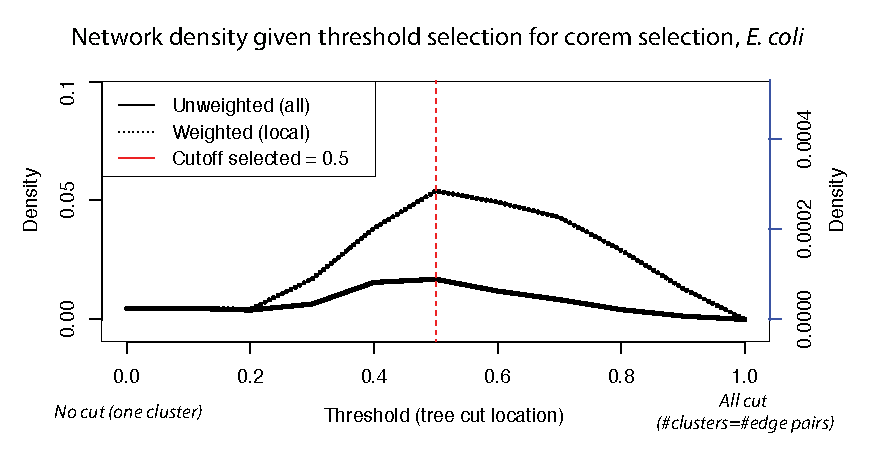
\includegraphics[width=0.9\linewidth]{figures/corem_density.pdf}
\caption[Corem density as a function of clustering cutoff threshold]{
{\bf Corem density as a function of clustering cutoff threshold.}
Hierarchical clustering cut threshold chosen to maximize the density
of resulting clusters. The cutoff chosen with modified weighted
density metric is identical to unweighted density metric.}
\label{fig:corem_density}
\end{figure}

Since the communities produced by this algorithm are comprised of sets
of edges, we defined a corem to include all genes incident to the
edges in a community. Because of this definition, each gene can be a
member of multiple different corems. In {\it H. salinarum}, this
procedure generated 679 corems ranging in size from 3 to 377 genes,
covering 1,363 of the 2,400 genes in the genome, and comprising 56,738
co-regulatory associations. In {\it E. coli}, we discovered 590
corems, ranging in size from 3 to 153 genes, covering 1,572 of 4,213
genes and 25,976 regulatory edges. See Table E1 and
Figure \ref{fig:corem_density} for additional
statistics. Gene-to-corem and corem-to-gene mappings for the {\it
H. salinarum} and {\it E. coli} models are available online.

\begin{figure}[hp]
\centering
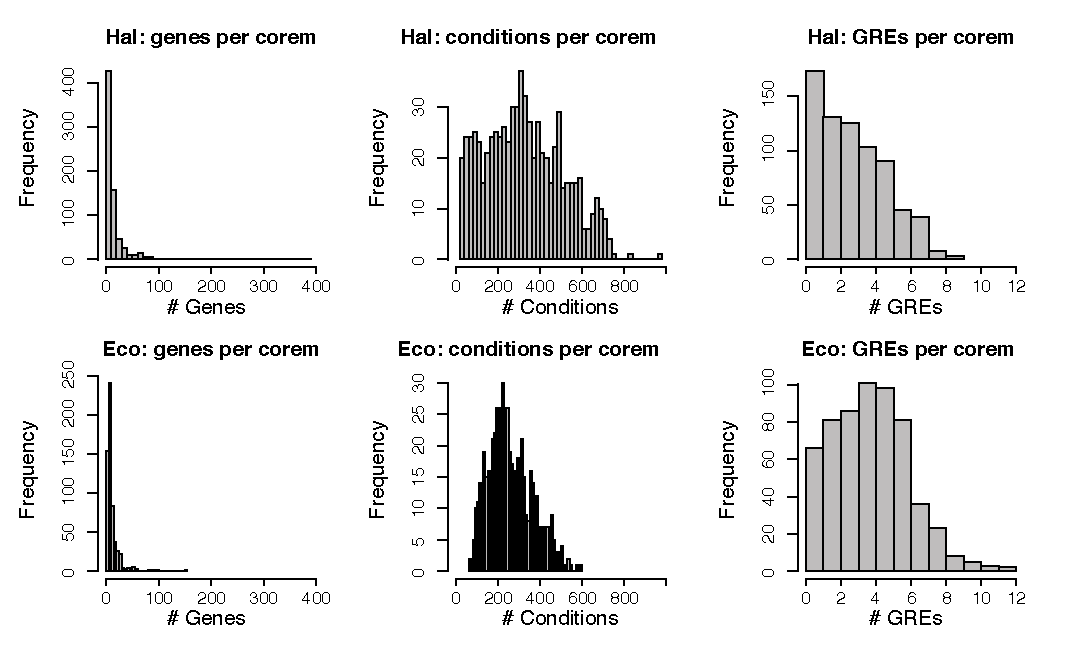
\includegraphics[width=0.9\linewidth]{figures/corem_stats.pdf}
\caption[Corem statistics]{
{\bf Corem statistics.} Number of genes, conditions, and GREs per
corem for \textit{E. coli} and \textit{H. salinarum} \egrine~models.}
\label{fig:corem_stats}
\end{figure}


\subsection{Functional enrichment estimates for genes in corems}

We computed functional enrichment for genes organized into corems
using DAVID (Dennis et al., 2003) and the DAVIDQuery R-package (Day
and Lisovich, 2010). Enrichments for each corem are available on the
web site.

\subsection{Conditional co-regulation of genes organized in corems}

We defined the conditions in which genes in a corem were co-regulated
as the set of experiments in which the genes of a corem are more
tightly co-expressed than one would expect at chance. We statistically
evaluated tight co-expression using relative standard deviation (RSD 
$=|\sigma/\mu|$) and resampling. We chose RSD (rather than, for example,
standard deviation, $\sigma$) to avoid over-weighting conditions in which the
mean relative expression is close to zero. The significance of an RSD
value for a given condition relative to each corem was estimated
by resampling: for a corem with $k$ gene members, and for each
condition, $c$, we computed at least 20,000 RSD values for $k$ randomly
sampled expression measurements in $c$, to determine the likelihood that the
observed co-expression has lower RSD than expected by chance ($p$-value
$< 0.01$). The resampling procedure resulted in condition sets for
corems that contained from 1.4\% to 85.5\% of the conditions in
\halo\ and 7.9\% to 66.6\% conditions in \eco.

\subsection{Conditionality of GRE influence}

The upstream promoter regions of most genes contain multiple EGRIN
2.0-predicted GREs (\eg, carA in Figure 2). A key insight of our
model is that not all of these sites are equally important for
controlling gene expression in all experimental conditions. We refer
to changes in the relative influence of GREs across conditions as
“conditional activity” of GRE elements. Although, to be clear, we do
not imply that the transcriptional activity at a GRE is attributable
to the DNA sequence itself, but rather the TF that binds to that
sequence in particular environments. We leveraged the GREs discovered
in genes grouped into corems and the conditional co-expression of
those groups of genes to predict conditionally active GREs in EGRIN
2.0.

Specifically, to discover active GREs for each corem we combined
predictions from (1) genome-wide motif scans (Section 5 above) that
predict the GRE locations in an expanded region around each gene’s
promoter in the corem using all of the ensemble predictions (1,000 nt
window: -875 nt upstream to 125 nt downstream), and (2) the conditions
discovered in biclusters that are most representative of the corem
(\ie, containing the largest fraction of genes from the corem, top
decile). GREs that occurred frequently in these biclusters were
considered putatively responsible for co-regulating the set of genes
in the condition-specific context of the corem (q-value ≤
0.05). Finally, we computed the average distances of all GREs to the
start codons of each gene in the list (collapsing sites if they
occurred within 25 nt of one another). The precise locations of all
GREs for the {\it H. salinarum} dpp operon-related corems (Figure 3) are
listed in Table E8, while the locations for GREs involved in
conditional modulation of the PurR regulon (Figure 4) are provided in
Table E9.

We represented the active GREs upstream of a gene or within a corem as
a pie chart, showing the normalized frequency with which the GREs
computed above occurred in biclusters containing that gene. For
example, if GREs 1, 2, and 3 occurred in 25, 50, and 200 biclusters
containing gene A, the pie chart for gene A would have sectors of area
0.09, 0.18, and 0.73 respectively. For corems, we computed the
normalized frequency of GREs for all genes of the corem. For example,
if GREs 1, 2, and 3 occurred in promoters of 10, 10, and 20 of the
genes of the corem, their areas would be 0.25, 0.25, and 0.5
respectively.

\subsection{Detection of conditional operons}

Conditional-specific transcriptional isoforms of operons were
predicted through corem membership. Specifically, if any of the genes
in an operon were found in a corem that did not contain all the other
genes of the operon, we predicted that the operon had conditional
isoforms. Operon annotations for both {\it H. salinarum} and {\it E. coli} were
derived from MicrobesOnline. All predicted conditional operons,
including the specific break sites and transcriptional isoforms is
available on the website. The full list of validated predictions is
provided in Table E7.

\subsection{Environmental ontology construction and usage}

We recorded a rich meta-data set for all 1495 experiments conducted
for {\it H. salinarum}. The meta-data includes a detailed description of
each experiment, including, for example: media composition, genetic
background, concentration of perturbant, internal reference batch id,
person who conducted the experiment, etc. We used this
meta-information to classify experiments in an ontological framework,
where two experiments can share specific meta-descriptions (\eg, 1e-3
mol/L EDTA), or inherit more general relationships from the
ontological structure (\eg, chemical perturbation). We used OBO-edit
to construct the ontology. The ontology contained 198 terms organized
across three primary branches (environmental state, experimental
state, and genetic state). The ontology flat file is available for
download and meta-data annotations for every array in the dataset are
available online.

We used the ontology to classify enriched environmental features for
GREs and corems (Figures 3-4). For corems, we used the set of
conditions in which genes in the corem are significantly co-expressed
(see 9 above) to compute term enrichment using the ontoCAT
R-package. Term enrichment was assessed statistically and reported as
q-values using the hypergeometric test with Benjamini-Hochberg
correction for multiple hypothesis testing.


\section{Model validation}\label{sec:validation}

\subsection{Global validation of gene regulatory elements predicted by \egrine}
\label{section:tfbs:vs:regdb}

We compared the genome-wide locations of predicted GREs in the {\it
  E. coli} \egrine~model to experimentally mapped TF binding sites
from \rdb~(BindingSiteSet table, filtered for experimental evidence
and TFs with $\geq 3$ unique binding sites; a total of 88 TFs). We
considered a GRE to be a significant match to a TF if a significant
fraction ($q$-value $\leq 0.05$) of its predicted non-coding locations
overlapped with the known binding locations for a particular TF
(hypergeometric $p$-value $\leq 0.01$; see GRE definition in
Section~\ref{section:gres}). In cases where a GRE significantly
matched multiple TFs, only the most significant was reported.

We observed several instances where more than one GRE significantly
matched the same TF. We were unable to determine whether this was the
result of incomplete GRE clustering, ambiguities related to GRE
scanning, limitations of the experimental data itself, or a reflection
of subtle context-dependent variations in the binding preferences of
these TFs. Since we did not observe clustering of GREs that map to the
same TF upon re-clustering, we hypothesize that the observations may
have biological origins, \ie, reflect condition-dependent variations
in TF binding preferences that are the result, for example, of
co-activator/repressor interaction or small molecule binding. It is
interesting to note that TFs with the largest fraction of GRE matches
include transcriptional dual regulators, such as FlhDC and UlaR (\ie,
TFs with the ability to act as both activators and repressors). This
is consistent with the observation that these TFs have
context-dependent binding preferences. The complete set of
validations, for both TFs and $\sigma$-factors, is listed in Table~E4.

\subsection{Global validation of regulatory interactions predicted by \egrine}
\label{section:aupr:vs:regdb}

We assessed the ability of the \egrine\ model to correctly infer known
regulatory interactions using the \rdb\ database as a standard metric
for comparison. Comparison to the \rdb\ gold-standard is common
practice for evaluating model performance \cite{Marbach2012}. We
performed our evaluation with the version of \rdb~ used by the DREAM5
ensemble (based on \rdb\ release 6.8 \cite{Marbach2012}) so that we
could directly compare our results. The authors \cite{Marbach2012}
restricted the gold-standard to well-established interactions,
annotated in \rdb\ with the `strong evidence' classification. In all
cases, networks were integrated from predictions among the ensemble
using an approach similar to that of \cite{Marbach2012}, with subtle
variations noted in each section, below. To facilitate a direct
comparison, we reconstructed a new {\it E. coli} \egrine\ model using
the same DREAM5 expression consortium as was used for the original
DREAM5 competition (Section~\ref{section:dream5_data_compendium}). The
predictions of this model were used {\it solely} for global validation
and direct comparison with the DREAM5 community network, as described
in this subsection.

We performed two global evaluations of the {\it E. coli} \egrine: (1)
a comparison of the GREs detected in the model with experimentally
mapped TF binding sites in \rdb~(Section~\ref{section:tfbs:vs:regdb}),
and (2) a comparison of the predicted (TF $\rightarrow$ gene) regulation
in \egrine~with the gene regulatory network from
\cite{Marbach2012}. For (2), we computed predicted regulatory networks
from \egrine~in two ways: (a) direct (TF $\rightarrow$ target)
predictions from \nwinf~ (Section~\ref{sec:nwinf_network}, and (b) a
gene regulatory network derived from predicted GREs that were matched
to TFs in
\rdb~(Section~\ref{section:gre_grn_construction}). Construction of
each of these networks is described in detail below
(Section~\ref{sec:nwinf_network} and
Section~\ref{section:gre_grn_construction}). The methods for, and
results of the comparisons are described in
Section~\ref{sec:network_comparisons}.

\subsubsection{Conversion of \egrine~\nwinf~influence predictions into a GRN}
\label{sec:nwinf_network}

We computed a direct (TF $\rightarrow$ gene) inferred {\it E. coli}
gene regulatory network (GRN) from the \nwinf~predictions in the
\egrine~ensemble. As with the original EGRIN model \cite{Bonneau2007},
\nwinf~influence predictions were originally made between the 296
putative {\it E. coli} TFs (Section \ref{section:eco_tfs}) and each of the
$\sim 40,000$ biclusters in the ensemble. We then used a weighted
average of the predicted influences among all networks in the
ensemble, as follows. If \nwinf~predicted a (TF $\rightarrow$
bicluster) influence with weight $\beta$ then we added $\beta$ to a
regulatory interaction between that TF and all genes in that
bicluster. Weights $\beta$ were summed for each recurrence of the same
(TF $\rightarrow$ gene) interaction. Note, we did not use $|\beta|$ in
the individual sums, since we considered contradicting evidence to be
cancelling rather than reinforcing. Finally, all (TF $\rightarrow$
gene) interactions in the final network were ranked by absolute total
weight (here we {\it did} use $|\beta|$). As with the DREAM5
competition networks, the top 100,000 rankings were retained in the
final network. The final \egrine~\nwinf~influence network is available
\href{http://egrin2.systemsbiology.net/}{online}.
%at \ref{tables:Inferelator_network.tsv}.

\subsubsection{Conversion of \egrine~GRE detections into a predicted GRN}
\label{section:gre_grn_construction}

We computed a separate inferred {\it E. coli} gene regulatory network
from predicted GREs in \egrine\ that were matched to TFs as described
in Section~\ref{section:tfbs:vs:regdb}. We would like to stress that
this inference relies upon (in this case, for {\it E. coli}) annotated
binding sites for regulators, which could be statistically linked to
predicted GREs through significant overlaps in their genomic
locations. This enables inference of (TF $\rightarrow$ gene) direct
influence predictions through the indirect relationship: 

\begin{equation}
\label{eq:gre_network_relation}
\mathrm{TF} \overset{\mathrm{anno.}}{\rightarrow} \mathrm{GRE} \overset{\mathrm{pred.}}{\rightarrow} \mathrm{gene}.
\end{equation}

\noindent Thus for an understudied organism, such as {\it
  H. salinarum}, such a network of (TF $\rightarrow$ gene) influences
could {\it not} be inferred; rather a (GRE $\rightarrow$ gene)
interaction network would be the final product. Such a network still
contains predictions which could be validated and acted upon, for
example, for engineering purposes. A future direction of our research
will be to statistically link TFs to predicted GREs, for example using
direct GRN predictions such as those described above
(\eg\ Section~\ref{sec:nwinf_network}, or \cite{Marbach2012}).

(GRE $\rightarrow$ gene) predictions (in
Eq.~\ref{eq:gre_network_relation}) were extracted from the
\egrine\ model directly using the \MEME\ predictions for motif
instances in the promoters of genes in each of the $\sim$40,000
\cm\ biclusters. We then used an unweighted average of the predictions
among all bicluster in the ensemble, as follows. A (TF $\rightarrow$
gene) edge with a weight of 1 was added to the predicted network if
the annotated binding sites for that TF could be matched with
locations of a motif (Section \ref{section:tfbs:vs:regdb}), which was
detected by \MEME\ in a bicluster in the promoter of the gene. Edge
weights (1) were added for each additional prediction, in the ensemble
of biclusters, of the same (TF $\rightarrow$ gene) interaction. As
with the \nwinf~influence network (Section \ref{sec:nwinf_network}), the top
100,000 rankings were retained in the final network. The final
\egrine~GRE-based network is available 
\href{http://egrin2.systemsbiology.net/}{online}.
%at \ref{tables:GRE_network.tsv}.

\subsubsection{Integration of predicted \egrine~\nwinf- and GRE-based GRNs}

Prior to integration of the two different predicted GRNs described
above (Sections~\ref{sec:nwinf_network}
and~\ref{section:gre_grn_construction}), we ensured that they were
both equally represented in the integrated GRN by re-scaling their
weights so that their sums would be equal. The GRNs were then combined
into a single, integrated predicted \egrine\ GRN by simply summing the
re-scaled weights for any edge predicted in both networks. Thus, this
final network integration was a form of weighted average of the two
(GRE and \nwinf) networks. This is {\it not} identical to the weighted
rank average method described by \cite{Marbach2012}, as it does not
use a posteriori assessments of each network to assign their relative
weights; rather the weights are simply adjust so that each network
contributes equally to the predictions.

\subsubsection{Network comparisons and global performance assessments}
\label{sec:network_comparisons}

To compare \egrine\ performance to the DREAM5 ensemble, we computed
standard precision-recall statistics for each network using the
previously described DREAM5 gold standard GRN.  We computed
area-under-the-precision-recall (AUPR) statistics to summarize the
predictive performance. AUPR statistics were compared directly with
the DREAM5 community ensemble network. By extension, the \egrine~AUPR
performance can be compared to the individual best performers in
DREAM5 as well (Figure~2A in \cite{Marbach2012}). The results of these
analyses are summarized in Figure~2A in the main text. We have made
all network predictions available
\href{http://egrin2.systemsbiology.net/}{online}. Complete
precision-recall curves are shown in Figure~\ref{fig:pr_curves}. The
curves are also available in tabular form
\href{http://egrin2.systemsbiology.net/}{online}.

\begin{figure}[h!]
\centering
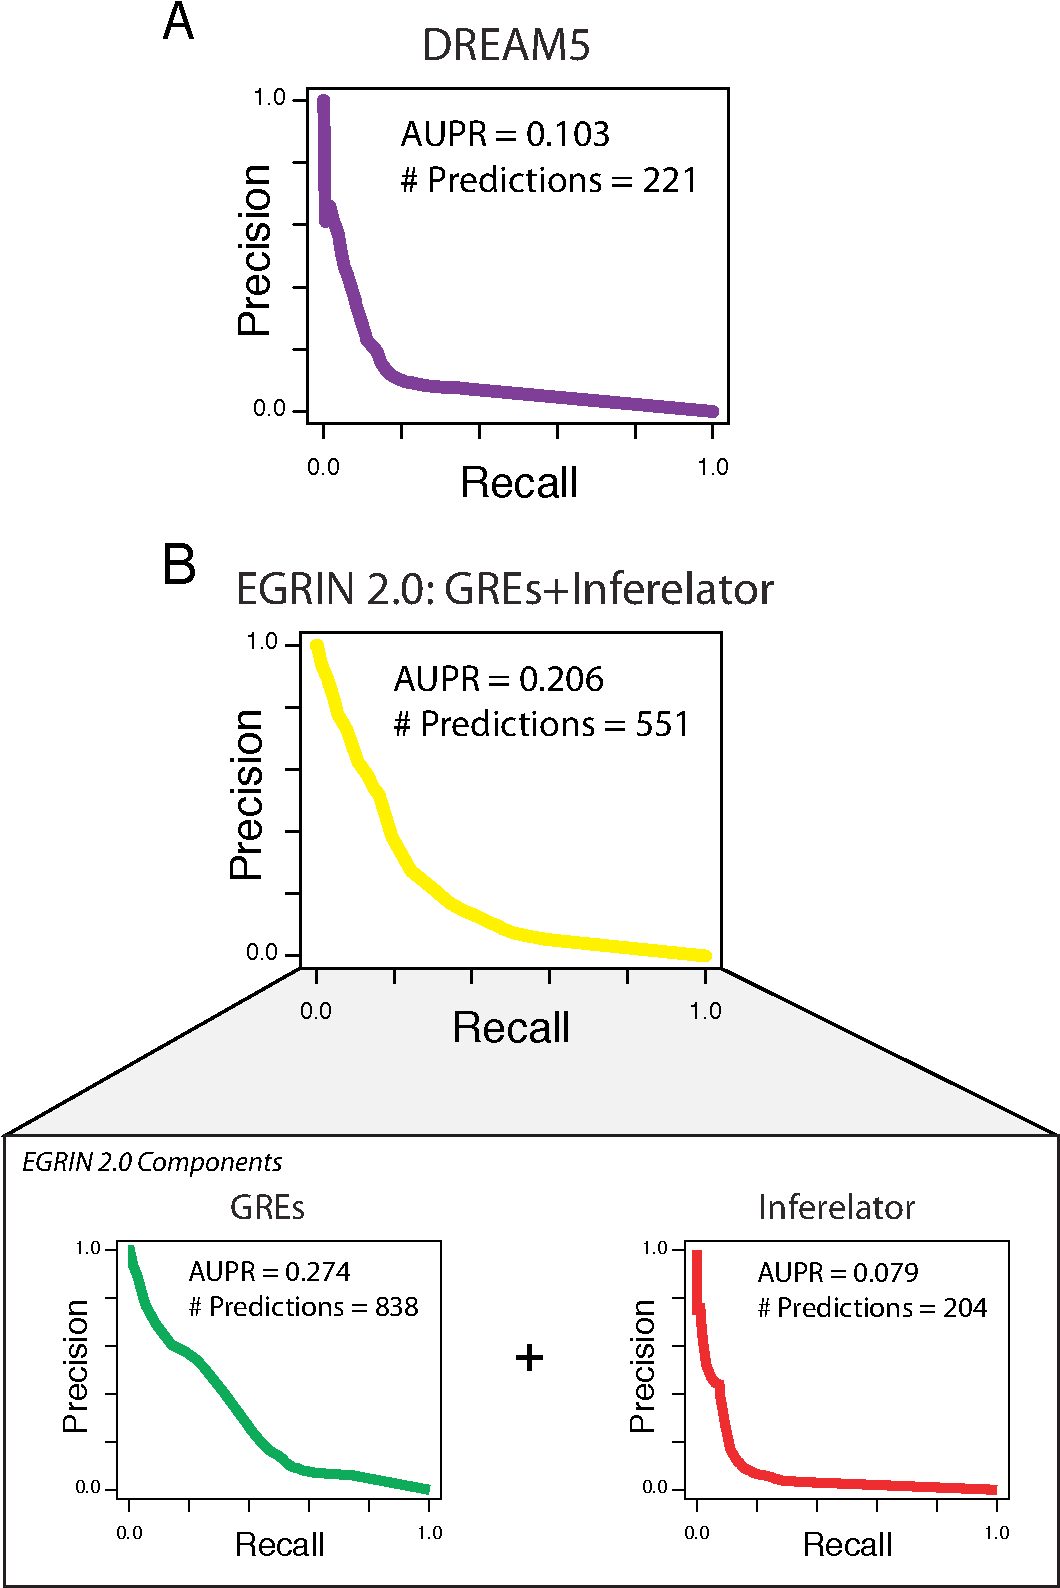
\includegraphics[width=0.5\linewidth]{figures/aupr.pdf}
\caption[Precision-recall performance for {\it E. coli}
  networks.]{\textbf{Precision-recall performance for \textit{E. coli}
    networks.} Comparison of precision-recall performance on {\it
    E. coli} \rdb~gold-standard (Section
  \ref{section:eco:gold:standard}), for the DREAM5 ensemble network
  (A), compared to \egrine (B).  We compare the GRE-based and
  \nwinf-based networks (bottom)to the integrated \egrine~network
  (top). The integrated \egrine~network consists of an equal weighting
  of the GRE-based and \nwinf-based networks.  The \egrine~networks
  were inferred using the DREAM5 mRNA expression compendium (Section
  \ref{section:dream5_data_compendium}). Area under the curve (AUPR)
  and the number of true-positive predictions at a precision of 25\%
  are listed for each curve.}
\label{fig:pr_curves}
\end{figure}

We further investigated the convergence of the AUPR statistics for
each of the \egrine-predicted regulatory networks as additional
individual EGRIN models are added to the ensemble. This assessment
helps to address the question of whether the approach utilized for
ensemble integration has the desired property of performing better
than most (if not all) of the individual models. Additionally, it can
address the question of how many individual EGRIN models are necessary
to achieve a given performance level. We observed that this is indeed
the case for the \nwinf-based predictions extracted from the
\egrine\ model (Figure~\ref{fig:cumulative_auprs}a), whose final AUPR
of 8.5\% far exceeds the rather poor performance of all 106 individual
component EGRIN models (with an average AUPR of 5.0\% and a maximum of
7.4\%). The performance of the ensemble for this measure converges
rather quickly to the final measure, after roughly 50 of the 106 EGRIN
models are integrated (taking into account the variance in models
observed with integrating the models in different orders).  For the
\egrine\ GRE-based predicted network
(Figure~\ref{fig:cumulative_auprs}b), ensemble surpasses 84 (79\%) of
the 106 individual component EGRIN models. This measure continues to
improve until $\sim 80$ of the 106 models are integrated, suggesting
that for this data set (the DREAM5 {\it E. coli} expression
compendium), $\sim 100$ EGRIN models was a reasonable number to use in
construction of the \egrine\ ensemble.

\begin{figure}[hp]
\centering
\mbox{
\subfigure[]{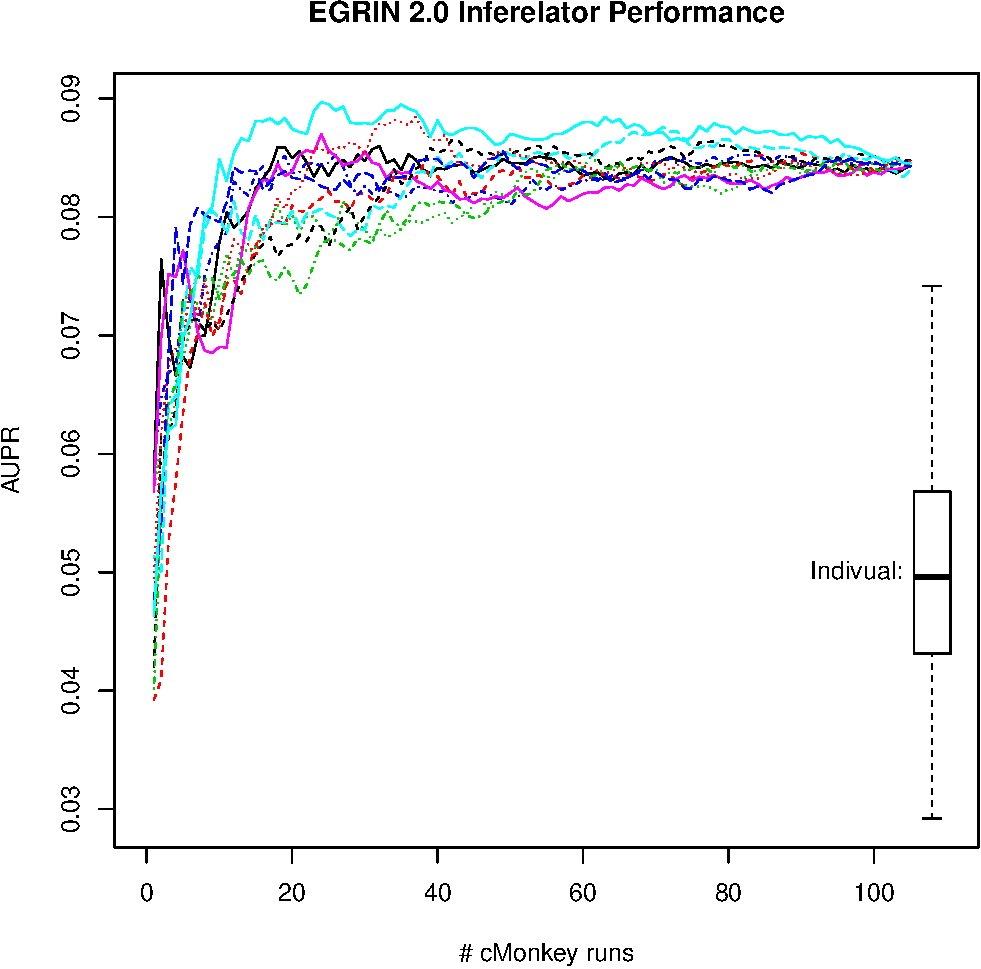
\includegraphics[width=0.4\linewidth]{figures/nwInf_cumulative_forPaper.pdf}}
\subfigure[]{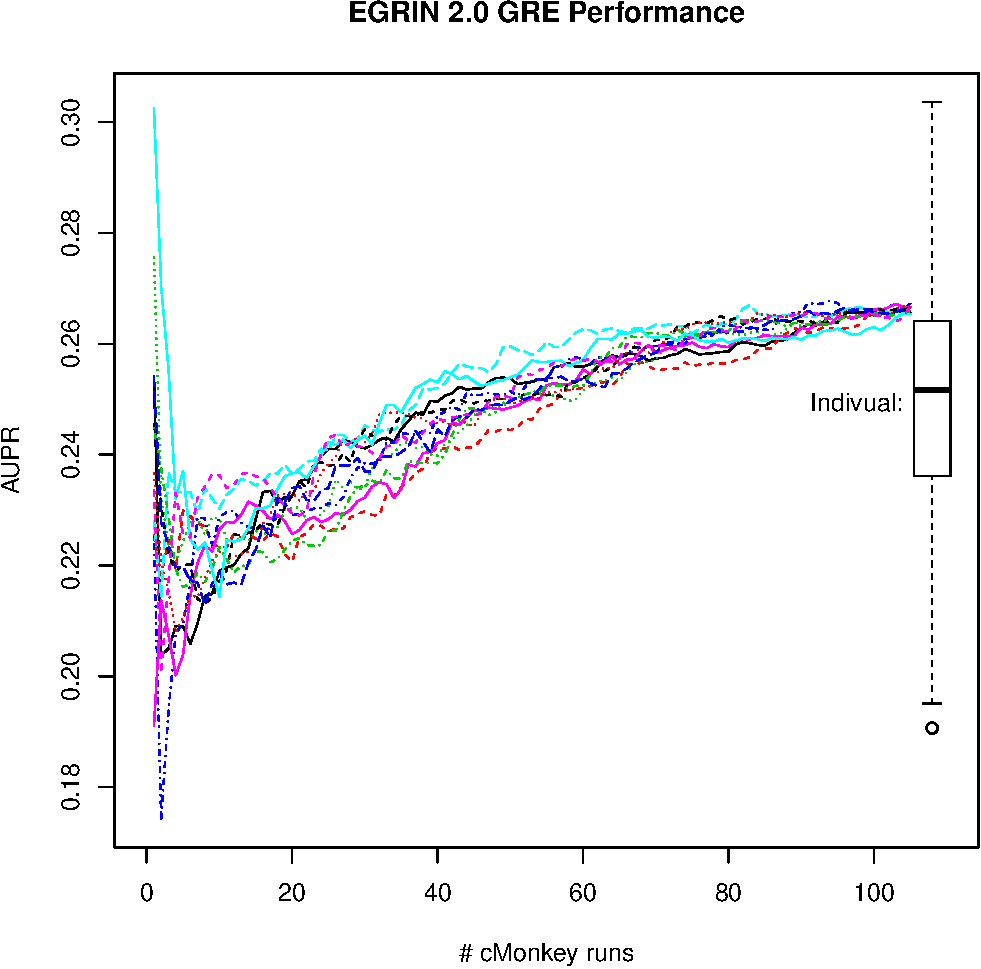
\includegraphics[width=0.4\linewidth]{figures/motif_cumulative_forPaper.pdf}}
}
\caption[Ensemble performance of individual GRN predictions]{
  \textbf{Ensemble performance of individual GRN predictions.}
  \egrine-inferred \textit{E. coli} regulatory network predictive
  performance (AUPR vs. {\it E. coli} DREAM5 \cite{Marbach2012} gold
  standard) for \nwinf-based predictions (a) and GRE-based predictions
  (b) from \egrine. Shown for both networks is the cumulative AUPR as
  each of the 106 individual model components is integrated in to the
  ensemble (as described in
  Section~\ref{section:aupr:vs:regdb}). Lines showing the cumulative
  AUPR for randomized orderings of the components' integration into
  the ensemble reveal the slight variations in performance that could
  be observed, and that these converge prior to integration of the
  final ($106^{\text{\tiny th}}$) component. Also included for
  comparison is a box-whisker plot which shows the distribution of
  corresponding AUPR scores for the 106 individual EGRIN models. }
\label{fig:cumulative_auprs}
\end{figure} 

Figure \ref{fig:argR_purR_networks} shows the inferred networks for
two genes regulated by PurR and ArgR (comparing predictions from
\egrine, \tmsamp{CLR}, DREAM5, and \tmsamp{RegPrecise} to the
annotations in \rdb). The result demonstrates that GRE-based
approaches can discover interactions that are not predicted using
direct approaches (See Section~\ref{section:gre_grn_construction}).

\begin{figure}[hp]
\centering
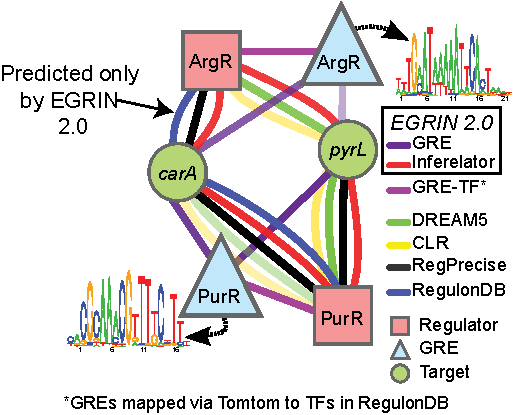
\includegraphics[width=0.5\linewidth]{figures/argR_purR_networks.pdf}
\caption[Integration of GRE discovery and \nwinf\ predictions
  yields comprehensive and detailed gene regulatory
  networks]{\textbf{Integration of GRE discovery and \nwinf\ 
    predictions yields comprehensive and detailed gene regulatory
    networks.} \egrine-inferred \textit{E. coli} regulatory subnetwork
  for two genes (green circles) in the PurR/ArgR regulon:
  \textit{carA} (\textit{b0032}) and \textit{pyrL} (\textit{b4246}).
  The \egrine~predictions are divided into GRE-based (dark violet) and
  \nwinf-based (red), and compared to predictions (or
  annotations) from other algorithms/databases (yellow: \tmsamp{CLR}; green:
  DREAM5 ensemble; black: \tmsamp{RegPrecise}; blue: \tmsamp{RegulonDB}). In two cases
  (ArgR$\rightarrow$carA and ArgR$\rightarrow$pyrL), \egrine~discovers
  regulatory interactions that were missed by either hand-curated
  databases or expression-based inference procedures.}
\label{fig:argR_purR_networks}
\end{figure} 

\subsection{Validation of condition-specific operon isoforms by tiling array transcriptome measurements}

We validated the prevalence of multiple, condition-specific
transcriptional isoforms from operons in \eco\ by measuring changes in
the transcriptome across growth, from lag-phase (OD600 = 0.05) to late
stationary phase (OD600 = 7.3). The experimental platform and other
experimental details are described in Section
\ref{section:ecoarray}. We used multivariate recursive partitioning,
including signals from both relative changes in expression along the
growth curve, as well as raw RNA hybridization signal to call putative
transcription breaks as previously described \cite{Koide2009}. To
determine the significance of our finding, we computed a $p$-value
describing the significance of the overlap between our predictions
(see Section \ref{section:condop}) and the experimental observations
using the cumulative hypergeometric distribution.

Figures \ref{fig:dpp_ecoli_expression}, \ref{fig:galE}, and
\ref{fig:ptsh} below depict several operons annotated with
condition-specific transcriptional isoforms. We have integrated GRE
elements discovered near break sites with the transcriptional
measurements.

\begin{figure}[hp]
\centering
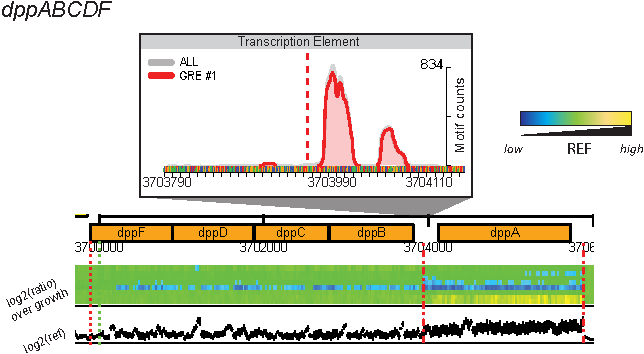
\includegraphics[width=0.7\linewidth]{figures/dpp_ecoli_expression.pdf}
\caption[GREs regulate multiple transcript isoforms from operons in
  {\it E. coli}, \textit{dppABCDF}]{\textbf{GREs regulate multiple
    transcript isoforms from operons in {\it E. coli},
    \textit{dppABCDF}.} GREs coincide with experimentally measured
  break sites. Three examples of experimentally determined
  transcription break sites (red dashed lines) in operons predicted by
  corems to be conditionally segmented. Expression levels of these
  regions were profiled across growth in rich media (heatmap). Inset
  contains region immediately surrounding a transcriptional break
  site, including counts of GREs discovered at these locations (as in
  Figure \ref{fig:nirH}).}
\label{fig:dpp_ecoli_expression}
\end{figure}

\begin{figure}[hp]
\centering
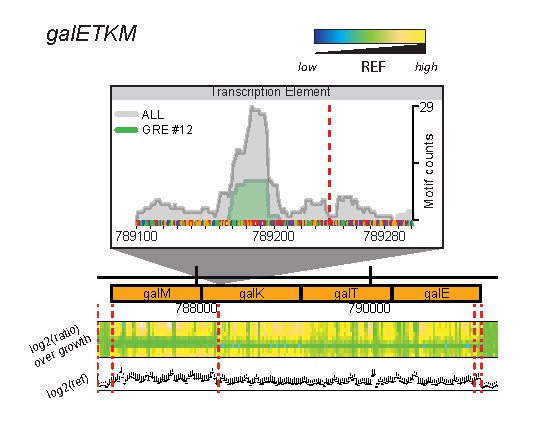
\includegraphics[width=0.7\linewidth]{figures/galE.pdf}
\caption[GREs regulate multiple transcript isoforms from operons in
  {\it E. coli}, \textit{galETKM}]{\textbf{GREs regulate multiple
    transcript isoforms from operons in {\it E. coli},
    \textit{galETKM}.} Caption details included in Figure
  \ref{fig:dpp_ecoli_expression}.}
\label{fig:galE}
\end{figure}

\begin{figure}[hp]
\centering
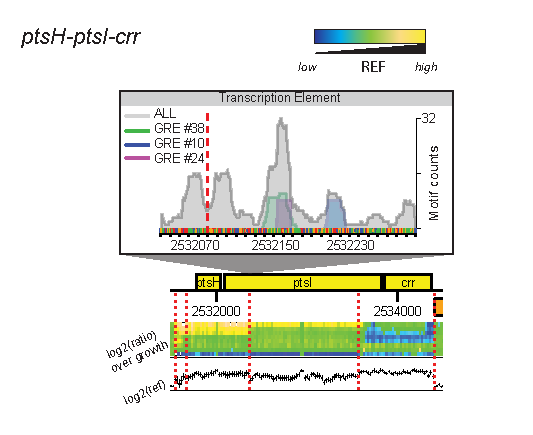
\includegraphics[width=0.7\linewidth]{figures/ptsh.pdf}
\caption[GREs regulate multiple transcript isoforms from operons in
  {\it E. coli}, \textit{ptsH-ptsI-crr}]{\textbf{GREs regulate
    multiple transcript isoforms from operons in {\it E. coli},
    \textit{ptsH-ptsI-crr}.} Caption details included in Figure
  \ref{fig:dpp_ecoli_expression}.}
\label{fig:ptsh}
\end{figure}

\subsection{Gene-gene co-fitness correlations in regulatory modules}

To assess the phenotypic consequences of co-regulation in corems, we
assessed whether genes grouped into corems had significantly similar
fitness consequences in many environments (\ie, the effect of deleting
one gene is highly similar to the effect of deleting the other across
many environments). We used the high-throughput fitness screen
described in Section \ref{section:fitness} to quantify these
relationships.

We compared the enrichment for high co-fitness relationships in corems
to other ways of assigning co-regulatory modules, including regulons
(\tmsamp{RegPrecise}, \rdb), operons, and \tmsamp{WGCNA}. The gene
modules for regulons (annotated in \rdb\ or \tmsamp{RegPrecise}
\cite{Novichkov2013}) consisted of genes annotated to a common TF. For
WGCNA, we assigned modules using the same community detection
procedures that we used to define corems from the \egrine~ensemble
(See \ref{section:gBg}). The gene co-expression modules were computed
from the weighted \tmsamp{WGCNA} adjacency matrix.

For the results presented in Figure~2B, we compared the distributions
of Pearson correlations between relative changes in fitness across
pairs of genes within each module, using the one-tailed
Kolmogorov-Smirnov test (KS-test). We report the KS $D$-statistic. The
precision/recall characteristics for each model are contained in Table~E5.

We extended this analysis by investigating whether the enriched high
co-fitness gene-gene relationships in corems consist of relationships
that could be described fully by regulons or operons. To answer this
question, we removed all gene pairs from corems that are also present
in operons or regulons and computed the KS-test again (Figure
\ref{fig:fitness_wo_operons}). We still observe a significant number
of high co-fitness relationships, suggesting that corems capture
physiologically meaningful co-regulatory relationships between genes
that cannot be explained by existing paradigms.

\begin{figure}[hp]
\centering
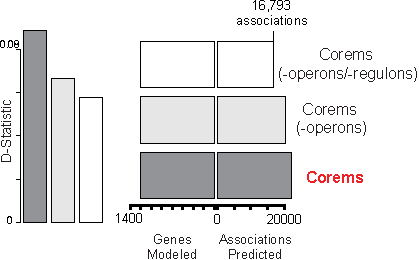
\includegraphics[width=0.6\linewidth]{figures/fitness_wo_operons.pdf}
\caption[\egrine~models highly correlated co-fitness relationships
  that cannot be explained by operons or
  regulons]{\textbf{\egrine~models highly correlated co-fitness
    relationships that cannot be explained by operons or regulons.}
  (Left) Enrichment for highly correlated, pairwise fitness
  measurements in gene knock outs across 324 conditions before and
  after removing gene associations annotated by operons
  (Microbes Online) and regulons (RegulonDB and RegPrecise)
  (KS-test,$D$-statistic). Two-thirds of gene-pairs with most highly
  correlated fitness within corems are not annotated by operons or
  regulons. (Right) Number of genes and associations predicted.}
\label{fig:fitness_wo_operons}
\end{figure}


\section{Model evaluation}\label{sec:evaluation}

In this section we evaluate the performance of the model as a function
of several important parameters. We focus in particular on how the
performance of the models changes as a function of the number of runs
included. From these evaluations, we conclude that (1) the model
performs well in its final form, (2) the model has reached a stable
state wherein inclusion of additional runs does not increase model
performance, and (3) the model is not over-fit to particular
experiments within a data set or to any data set as a whole.

\subsection{Comparison with other module detection algorithms}

We compared the number of \rdb~TFs detected in the \egrine~model to individual
\cm~runs as well as to several other module detection/clustering
algorithms that were computed on subsets of the experimental data
(similar to the \egrine~ensemble; Figure \ref{fig:motclust}). We
evaluated: (a) $k$-means clustering, (b) \tmsamp{WGCNA}
\cite{Langfelder2008}, and (c) \tmsamp{DISTILLER}
\cite{Lemmens2009}. For (a) and (b), we computed modules 100 times on
random subsets of the {\it E. coli} expression data set (using 200-250
randomly chosen experiments per run; selection criteria were identical
to {\it E. coli} \egrine; see Table~\ref{tab:cmparams:eco}). We then
predicted {\it de novo cis}-regulatory GREs in the promoter regions of genes
in each module using \tmsamp{MEME} (\tmsamp{MEME} parameters were also
identical to \egrine; Table~\ref{tab:cmparams:eco}). For (c), we
performed the comparison using the original modules generated by
\cite{Lemmens2009}. Rather than alter module composition by
re-detection, we instead varied \tmsamp{MEME} parameters applied to
the modules 100 times (again, within the same ranges as those used for
\egrine). TF-GRE matches were assigned by comparing GREs to
\rdb~TF binding sites, as previously described
(Section~\ref{section:tfbs:vs:regdb}).

We found that individual \cm~runs discovered a greater number of
\rdb~binding sites, on average, than the other methods (an average of
41 for \cm, compared to averages of 30, 25, and 29 for $k$-means,
\tmsamp{WGCNA}, and \tmsamp{DISTILLER}, respectively), which is
consistent with previous findings \cite{Reiss2006n}
(Figure~\ref{fig:ensemble_comparison_regDB}). Integration of all
\cm~biclusters into the complete \egrine~ensemble outperformed all
individual \cm~runs (53 total, as described in the Manuscript). This
result is typical of ensemble-based inference approaches, and supports
value of ensemble integration as part of the \egrine~ model.

\begin{figure}[h!]
\centering
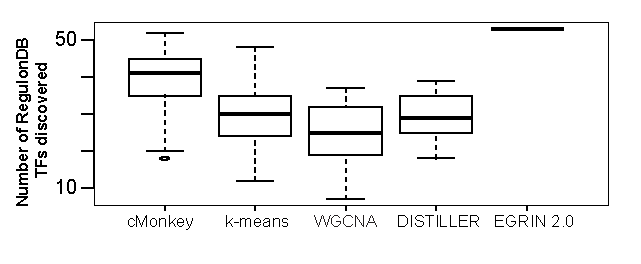
\includegraphics[width=0.95\linewidth]{figures/ensemble_comparison_regDB.pdf}
\caption[Number of TFs in \rdb~ re-discovered by various
    regulatory module detection methods.]  {{\bf Number of TFs in
    \rdb~ re-discovered by various regulatory module detection
    methods.} Comparison of \egrine~ (solid line, far right) to
  individual \cm\ runs, as well as multiple runs of $k$-means,
  \tmsamp{WGCNA}, and \tmsamp{DISTILLER} on subsets of the expression
  data. Evaluation made with respect to re-discovery of binding sites
  for 88 TFs with $\geq 3$ unique sites in \rdb~ based on genome-wide
  binding site locations (FDR $\leq 0.05$).}
\label{fig:ensemble_comparison_regDB}
\end{figure}

\subsection{Convergence and stability of the inferred network}

To evaluate the stability of the inferred \egrine network, we
quantified how the model changes as the underlying cMonkey models used
to construct the ensemble are altered. Since sub-bagging acts
similarly to cross-validation, we viewed this as an opportunity to
evaluate whether the model is over-fit to particular experiments in
the data set. Specifically, we asked how many runs are required to
converge on a consistently inferred network, i.e., where the inferred
gene-gene co-occurrence matrix is largely identical (see Section
\ref{}). In Figure \ref{fig:gBg_network_converge} we demonstrate
the. This means that even with

\begin{figure}[h!]
\centering
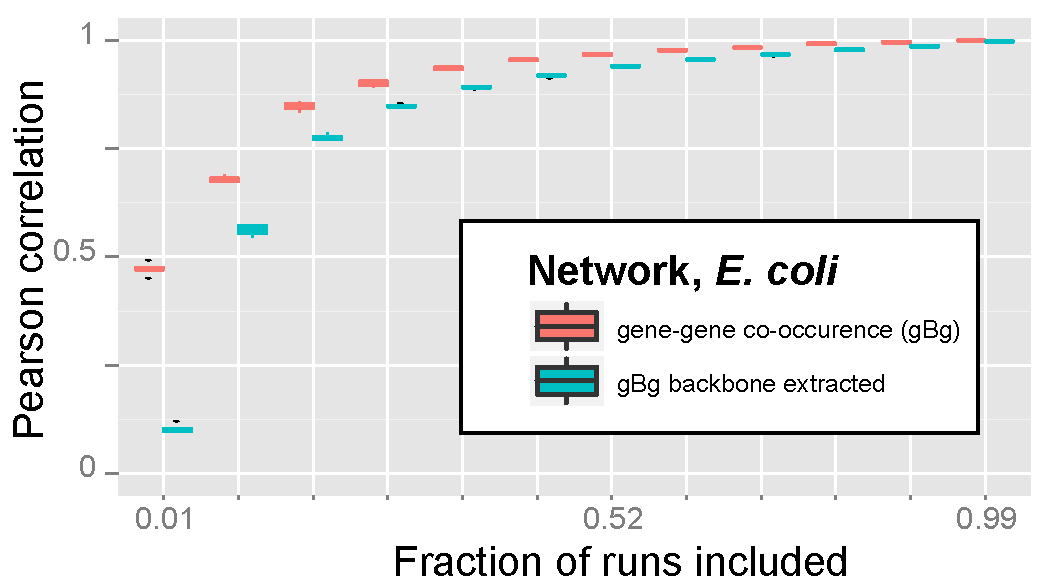
\includegraphics[width=0.75\linewidth]{figures/gBg_network_converge.pdf}
\caption[Convergence of \egrine inferred networks.]  {{\bf Convergence of \egrine inferred networks.}} 
\label{fig:gBg_network_converge}
\end{figure}

\subsection{Discovery of corems in an independent data set}

To determine whether the overfit 

\begin{figure}[h!]
\centering
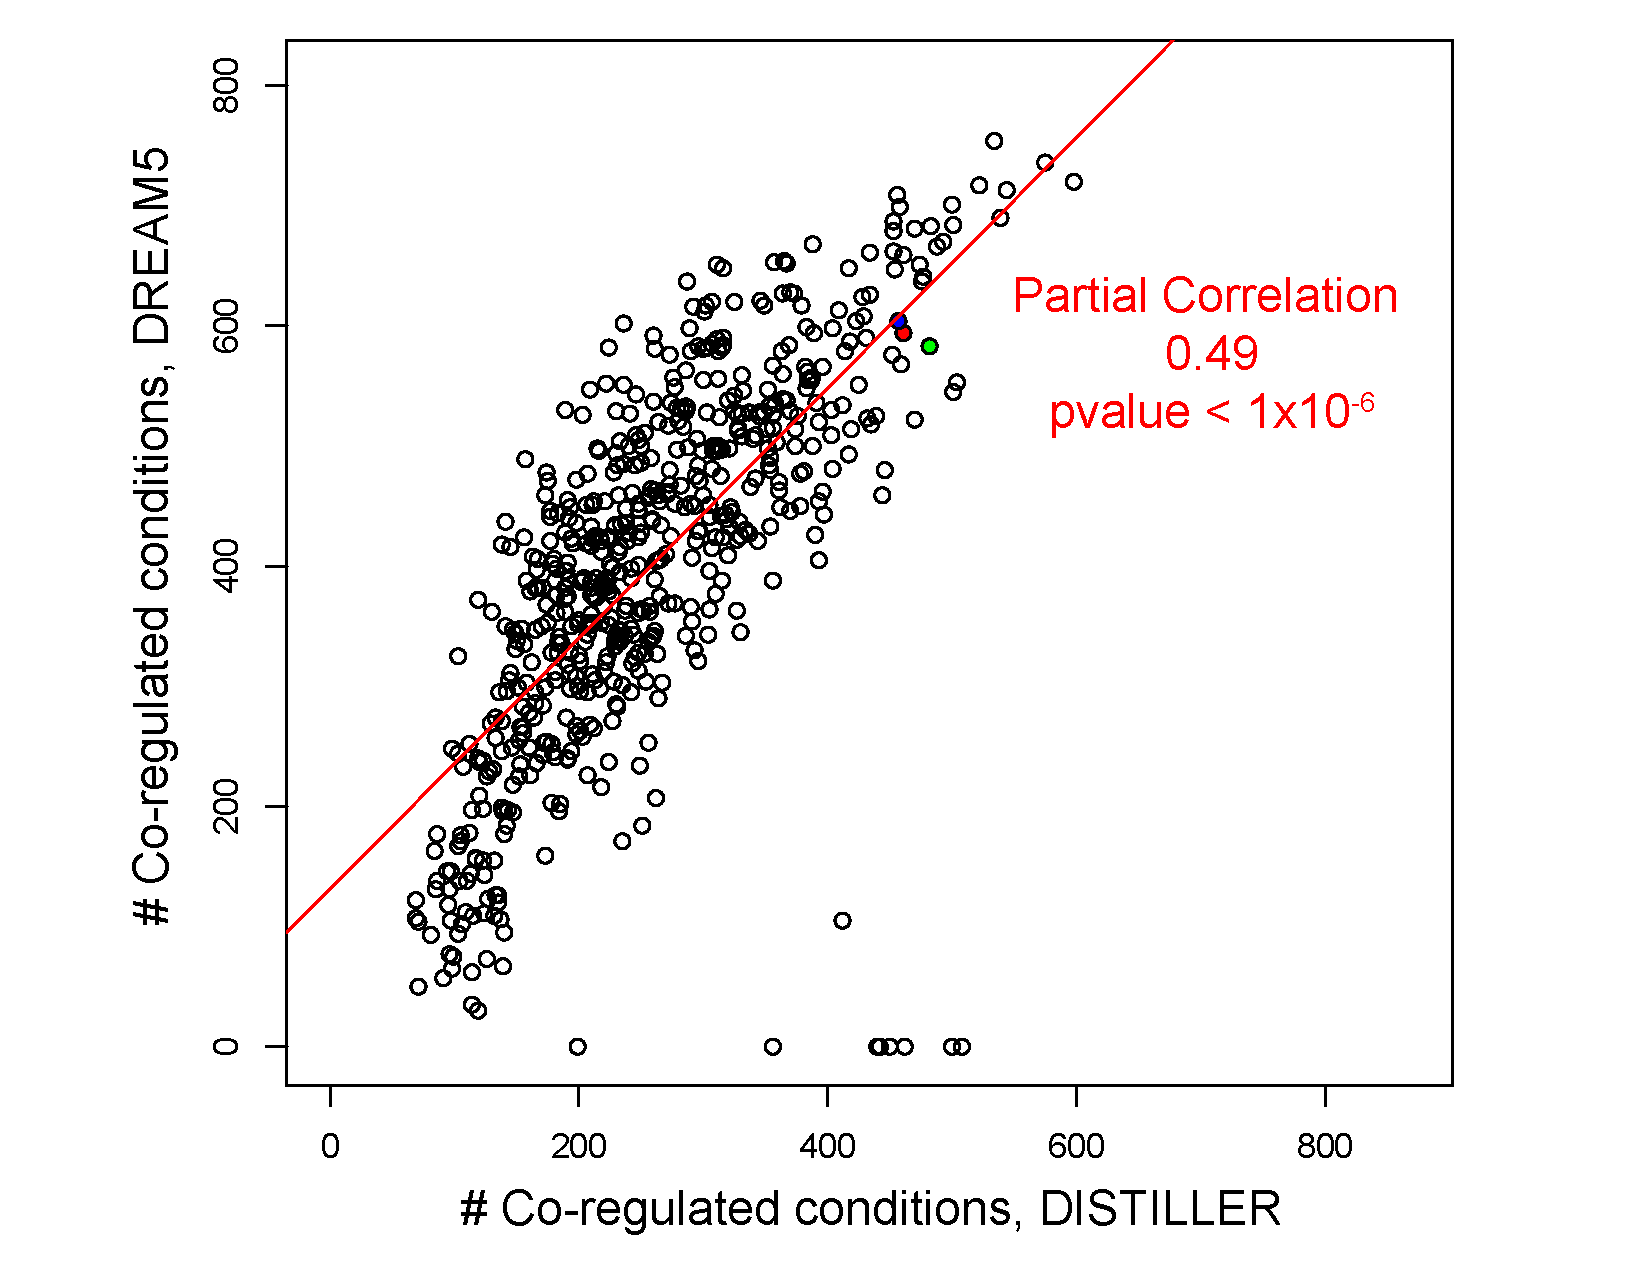
\includegraphics[width=0.75\linewidth]{figures/corem_conds_distiller_dream5.pdf}
\caption[Number of TFs in \rdb~ re-discovered by various
    regulatory module detection methods.]  {{\bf Number of TFs in
    \rdb~ re-discovered by various regulatory module detection
    methods.} Comparison of \egrine~ (solid line, far right) to
  individual \cm\ runs, as well as multiple runs of $k$-means,
  \tmsamp{WGCNA}, and \tmsamp{DISTILLER} on subsets of the expression
  data. Evaluation made with respect to re-discovery of binding sites
  for 88 TFs with $\geq 3$ unique sites in \rdb~ based on genome-wide
  binding site locations (FDR $\leq 0.05$).}
\label{fig:corem_conds_distiller_dream5}
\end{figure}



\section{Additional Supporting Figures Referenced From Main Text}

\label{suppfigs}

\DIFdelbegin %DIFDELCMD < \begin{enumerate}
%DIFDELCMD < \item %%%
\DIFdel{Supplementary Figure~\ref{fig:workflow}
}%DIFDELCMD < \item %%%
\DIFdel{Supplementary Figure~\ref{fig:motclust}
}%DIFDELCMD < \item %%%
\DIFdel{Supplementary Figure~\ref{fig:fitness}
}%DIFDELCMD < \item %%%
\DIFdel{Supplementary Figure~\ref{fig:gresVsOperons}
}%DIFDELCMD < \item %%%
\DIFdel{Supplementary Figure~\ref{fig:corems}
}%DIFDELCMD < \item %%%
\DIFdel{Supplementary Figure~\ref{fig:suppfig6}
}%DIFDELCMD < \end{enumerate}
%DIFDELCMD < 

%DIFDELCMD < \begin{figure}[!b]
%DIFDELCMD < %%%
\DIFdelend \DIFaddbegin \begin{figure}[hp]
\DIFaddendFL \centering
\DIFdelbeginFL %DIFDELCMD < \epsfig{file=figures/e1.eps,width=0.95\linewidth}
%DIFDELCMD < %%%
%DIF < \\\\\vspace{.07in}\hline\\\\\vspace{.07in}
%DIFDELCMD < \caption{{\bf %%%
\DIFdelFL{Detailed workflow for EGRIN 2.0 inference
procedure.}%DIFDELCMD < } %%%
\DIFdelFL{Data input, processing and analysis to construct EGRIN 2.0
model for }%DIFDELCMD < {\it %%%
\DIFdelFL{H. salinarum}%DIFDELCMD < } %%%
\DIFdelFL{and }%DIFDELCMD < {\it %%%
\DIFdelFL{E. coli}%DIFDELCMD < }%%%
\DIFdelFL{, and predictions
generated. Predictions highlighted in individual figures are noted.}%DIFDELCMD < }
%DIFDELCMD < \label{fig:workflow}
%DIFDELCMD < \vspace{-.1in}
%DIFDELCMD < %%%
\DIFdelendFL \DIFaddbeginFL 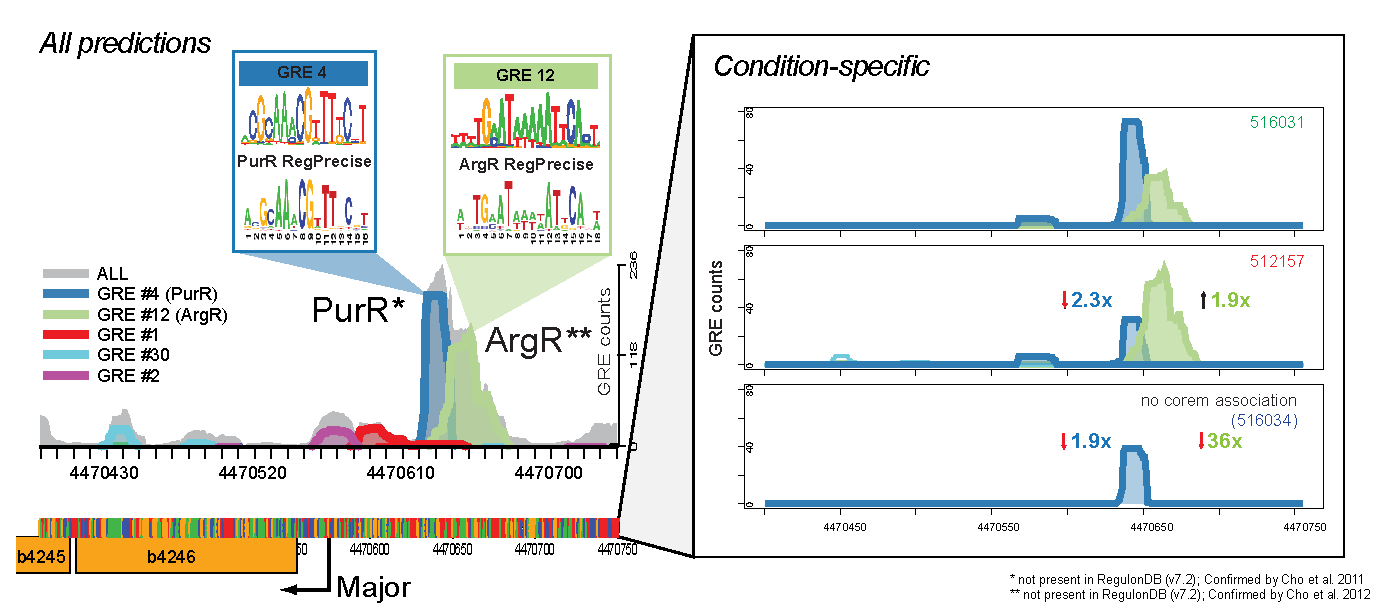
\includegraphics[width=0.95\linewidth]{figures/pyrL.pdf}
\caption[Differential GRE activity in \textit{pyrL} promoter, \textit{E. coli}]{\textbf{\DIFaddFL{Differential GRE activity in }\textit{\DIFaddFL{pyrL}} \DIFaddFL{promoter, }\textit{\DIFaddFL{E. coli}}\DIFaddFL{.}} \DIFaddFL{(Left) Predicted promoter architecture for }{\it \DIFaddFL{E. coli}} \textit{\DIFaddFL{pyrL}} \DIFaddFL{(}\textit{\DIFaddFL{b4246}}\DIFaddFL{). Overlapping GREs matching to PurR (GRE }\#\DIFaddFL{4) and ArgR (GRE }\#\DIFaddFL{12) were detected upstream of pyrL. These sites were not annotated in RegulonDB, but were validated in independent ChIP-chip experiments \mbox{%DIFAUXCMD
\cite{Cho2012,Cho2011a}
}%DIFAUXCMD
. Transcription start site indicated with arrow. (Bottom) Condition-specific promoter architectures for }{\it \DIFaddFL{E. coli}} \textit{\DIFaddFL{pyrL}} \DIFaddFL{(as in Figure 2E). Variation in predicted GRE activity across three different subsets of experimental conditions (counts and fold-change) for two GREs in the }\textit{\DIFaddFL{pyrL}} \DIFaddFL{promoter. Experimental subsets correspond to conditions under which at least one of three nucleotide biosynthetic corems is regulated (denoted by colored names at top-right of each plot)}}
\label{fig:pyrL}
\DIFaddendFL \end{figure}

\DIFdelbegin %DIFDELCMD < \begin{figure}[!b]
%DIFDELCMD < %%%
\DIFdelend \DIFaddbegin \begin{figure}[hp]
\DIFaddendFL \centering
\DIFdelbeginFL %DIFDELCMD < \epsfig{file=figures/e2.eps,width=0.8\linewidth}
%DIFDELCMD < %%%
%DIF < \\\\\vspace{.07in}\hline\\\\\vspace{.07in}
%DIFDELCMD < \caption{{\bf %%%
\DIFdelFL{Genome-wide discovery and validation of gene
regulatory elements (}\DIFdelendFL \DIFaddbeginFL 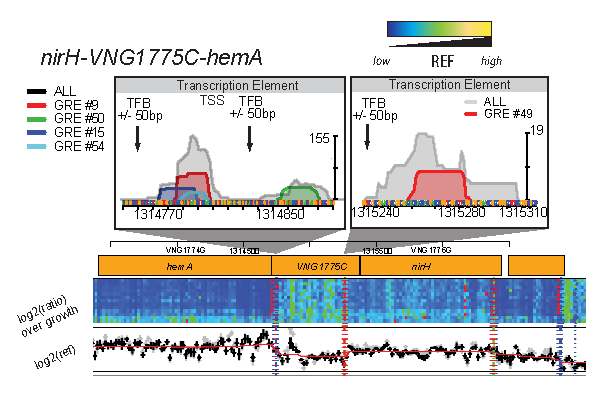
\includegraphics[width=0.95\linewidth]{figures/nirH.pdf}
\caption[GREs regulate multiple transcript isoforms from operons in {\it H. salinarum}, \textit{nirH-VNG1775C-hemA}.]{\textbf{\DIFaddFL{GREs regulate multiple transcript isoforms from operons in }{\it \DIFaddFL{H. salinarum}}\DIFaddFL{, }\textit{\DIFaddFL{nirH-VNG1775C-hemA}}\DIFaddFL{.}} \DIFaddendFL GREs \DIFdelbeginFL \DIFdelFL{). (A) Motif clustering and GRE
identification.}%DIFDELCMD < } %%%
\DIFdelFL{(Left) A schematic of the approach used to align and
cluster individually detected motifs to define GREs. In this example,
similar motifs were aligned and clustered into three GREs using Tomtom
and mcl (Details in Methods and Supplementary Methods). (Center) The
}%DIFDELCMD < {\it %%%
\DIFdelFL{H. salinarum}%DIFDELCMD < } %%%
\DIFdelFL{network of aligned and clustered motifs. (Right)
Two }%DIFDELCMD < {\it %%%
\DIFdelFL{H. salinarum}%DIFDELCMD < } %%%
\DIFdelFL{GREs discovered by this method. The motif logo
of each GRE was generated by summing PSSMs of the individual aligned
motifs in the cluster, as illustrated by three examples of individual
motifs (prior to alignment) for each of the two GREs. Note that
relative to the individual motifs, the averaged GRE motif is more
palindromic - a hallmark of binding sites for dimeric TFs. }%DIFDELCMD < {\bf %%%
\DIFdelFL{(B)
Integration of GRE discovery and Inferelator predictions yields
comprehensive and detailed gene regulatory networks.}%DIFDELCMD < } %%%
\DIFdelFL{EGRIN
2.0-inferred }%DIFDELCMD < {\it %%%
\DIFdelFL{E. coli}%DIFDELCMD < } %%%
\DIFdelFL{regulatory subnetwork for two genes (green
circles) in the PurR/ArgR regulon: carA (b0032) and pyrL (b4246).  The
EGRIN 2.0 predictions are divided into GRE-based (dark violet) and
Inferelator-based (red), and compared to predictions (or annotations)
from other algorithms/databases (yellow: CLR; green: DREAM5 ensemble;
black: RegPrecise; blue: RegulonDB). In two cases
(ArgR$\rightarrow$carA and ArgR$\rightarrow$pyrL), EGRIN 2.0 discovers
regulatory interactions that were missed by either hand-curated
databases or expression-based inference procedures. }%DIFDELCMD < {\bf %%%
\DIFdelFL{(C) Number of TFs
in RegulonDB re-discovered by various methods.}%DIFDELCMD < } %%%
\DIFdelFL{Comparison of EGRIN 2.0
(solid line, far right) to individual }%DIFDELCMD < \cm\ %%%
\DIFdelFL{runs, as well as
multiple runs of k-means, WGCNA, and DISTILLER on subsets of the
expression data. Evaluation made with respect to re-discovery of 88
TFs in RegulonDB with $\geq 3$ unique sites based on genome-wide
binding site locations (FDR $\leq 0.05$). }%DIFDELCMD < {\bf %%%
\DIFdelFL{(D) Genome-wide
distribution of GREs relative to experimentally mapped transcriptional
start sites in }%DIFDELCMD < {\it %%%
\DIFdelFL{H. salinarum}%DIFDELCMD < }%%%
\DIFdelFL{.}%DIFDELCMD < } %%%
\DIFdelFL{(Left) Predicted positions for all GREs
in gene promoters upstream of experimentally mapped transcription
start sites (TSSs; Koide et al., 2009) in and (Right) four example
elements. Distribution peaks for most GREs occur at characteristic
locations. For instance, the location of TATA box-like elements
(GRE }%DIFDELCMD < \#%%%
\DIFdelFL{25) between -21 to -40 nt upstream to TSSs in }%DIFDELCMD < {\it %%%
\DIFdelFL{H. salinarum}%DIFDELCMD < } %%%
\DIFdelFL{is
consistent with the characterized location of basal elements in
archaeal promoters (-25 to 30 nt upstream to TSS). GRE location
enables prediction of putative roles for the cognate TF (}%DIFDELCMD < \eg
%DIFDELCMD < %%%
\DIFdelFL{repressor, activator or a basal factor).}%DIFDELCMD < }
%DIFDELCMD < \label{fig:motclust}
%DIFDELCMD < \vspace{-.1in}
%DIFDELCMD < \end{figure}
%DIFDELCMD < 

%DIFDELCMD < \begin{figure}[!b]
%DIFDELCMD < \centering
%DIFDELCMD < \epsfig{file=figures/e3.eps,width=0.95\linewidth}
%DIFDELCMD < %%%
%DIF < \\\\\vspace{.07in}\hline\\\\\vspace{.07in}
%DIFDELCMD < \caption{{\bf %%%
\DIFdelFL{EGRIN 2.0 models dynamic regulatory mechanisms that
    result in highly correlated fitness effects.}%DIFDELCMD < }  
%DIFDELCMD < {\bf %%%
\DIFdelFL{(A)}%DIFDELCMD < } %%%
\DIFdelFL{(Left) Enrichment for highly correlated, pairwise fitness
  measurements in gene knock outs across 324 conditions before and
  after removing gene associations annotated by operons
  (MicrobesOnline) and regulons (RegulonDB and RegPrecise) (KS-test,
  $D$-statistic). Two-thirds of gene-pairs with most highly correlated
  fitness within corems are not annotated by operons or
  regulons. (Right) Number of genes and associations predicted. }%DIFDELCMD < {\bf %%%
\DIFdelFL{(B)
  Deciphering GREs responsible for regulating corems.}%DIFDELCMD < } %%%
\DIFdelFL{A GRE is
  implicated in regulation of a corem when it is both (1) }\DIFdelendFL located \DIFdelbeginFL \DIFdelFL{within an expanded region (-875nt to +125nt) around the translation
  start site of any gene in the corem; and (2) present in biclusters
  containing a large fraction of corem genes (top decile). Relative
  GRE influence is computed as the frequency with which each GRE was
  discovered in these representative biclusters (see Supplementary
  Methods for more details). Influence scores are illustrated as pie
  charts and reported for each gene individually (}%DIFDELCMD < \eg%%%
\DIFdelFL{, VNG2347G); and
  as a composite by averaging across all genes in a corem. The width
  of each sector in the pie charts is proportional to the frequency of
  GRE discovery.  }%DIFDELCMD < {\bf %%%
\DIFdelFL{(C)}%DIFDELCMD < } %%%
\DIFdelFL{(Top) Predicted promoter architecture for
  }%DIFDELCMD < {\it %%%
\DIFdelFL{E. coli}%DIFDELCMD < } %%%
\DIFdelFL{pyrL (b4246). Overlapping GREs matching to PurR (GRE }%DIFDELCMD < \#%%%
\DIFdelFL{4) and
  ArgR (GRE }%DIFDELCMD < \#%%%
\DIFdelFL{12) were detected upstream of pyrL. These sites were not
  annotated in RegulonDB, but were validated in independent ChIP-chip
  experiments (Cho et al., 2012; Cho et al., 2011). Transcription
  start site indicated with arrow. (Bottom) Condition-specific
  promoter architectures for }%DIFDELCMD < {\it %%%
\DIFdelFL{E. coli}%DIFDELCMD < } %%%
\DIFdelFL{pyrL (as in Figure 2E). Variation
  in predicted GRE activity across three different subsets of
  experimental conditions (counts and fold-change) for two GREs in the
  pyrL promoter. Experimental subsets correspond to conditions under
  which at least one of three nucleotide biosynthetic corems is
  regulated (denoted by colored names at top-right of each plot) }%DIFDELCMD < }
%DIFDELCMD < \label{fig:fitness}
%DIFDELCMD < \vspace{-.1in}
%DIFDELCMD < \end{figure}
%DIFDELCMD < 

%DIFDELCMD < \begin{figure}[!b]
%DIFDELCMD < \centering
%DIFDELCMD < \epsfig{file=figures/e4.eps,width=0.95\linewidth}
%DIFDELCMD < %%%
%DIF < \\\\\vspace{.07in}\hline\\\\\vspace{.07in}
%DIFDELCMD < \caption{{\bf %%%
\DIFdelFL{GREs regulate internal modulation of operons in
    }%DIFDELCMD < {\it %%%
\DIFdelFL{H. salinarum}%DIFDELCMD < }%%%
\DIFdelFL{.}%DIFDELCMD < }  {\bf %%%
\DIFdelFL{(A) GREs located }\DIFdelendFL inside operons coincide with experimentally measured transcriptional break sites. \DIFdelbeginFL %DIFDELCMD < } %%%
\DIFdelendFL Experimentally determined transcription break sites (red dashed lines) above expression profiles of these regions across growth (heatmap, \DIFdelbeginFL \DIFdelFL{Koide
  et al., 2009) }\DIFdelendFL \DIFaddbeginFL \DIFaddFL{\mbox{%DIFAUXCMD
\cite{Koide2009}
}%DIFAUXCMD
}\DIFaddendFL and ChIP-chip TFBs (\DIFdelbeginFL \DIFdelFL{Facciotti et al.}\DIFdelendFL \DIFaddbeginFL \DIFaddFL{\mbox{%DIFAUXCMD
\cite{Facciotti2007}
}%DIFAUXCMD
}\DIFaddendFL , \DIFdelbeginFL \DIFdelFL{2007, }\DIFdelendFL vertical arrows) support the role of GREs in regulating segmentation of the operon in certain conditions. Insets contain regions immediately surrounding transcriptional break sites, including counts of GREs discovered at these locations.\DIFdelbeginFL \DIFdelFL{Three examples of conditionally
  segmented operons are shown. }%DIFDELCMD < {\bf %%%
\DIFdelFL{(B) Alternate regulatory modes for dpp
  operon predicted by corems.}%DIFDELCMD < } %%%
\DIFdelendFL \DIFaddbeginFL }
\label{fig:nirH}
\end{figure}

\begin{figure}[hp]
\centering
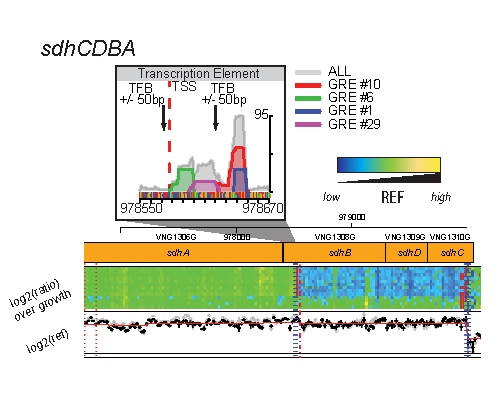
\includegraphics[width=0.95\linewidth]{figures/sdh.pdf}
\caption[GREs regulate multiple transcript isoforms from operons in {\it H. salinarum}, \textit{sdhCDBA}.]{\textbf{\DIFaddFL{GREs regulate multiple transcript isoforms from operons in }{\it \DIFaddFL{H. salinarum}}\DIFaddFL{, }\textit{\DIFaddFL{sdhCDBA}}\DIFaddFL{.}} \DIFaddFL{Caption details included in Figure \ref{fig:nirH}}}
\label{fig:sdh}
\end{figure}

\begin{figure}[hp]
\centering
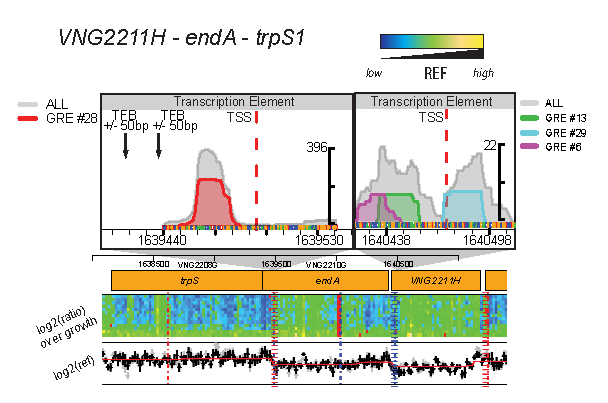
\includegraphics[width=0.95\linewidth]{figures/vng2211h.pdf}
\caption[GREs regulate multiple transcript isoforms from operons in {\it H. salinarum}, \textit{VNG2211H-endA-trpS1}.]{\textbf{\DIFaddFL{GREs regulate multiple transcript isoforms from operons in }{\it \DIFaddFL{H. salinarum}}\DIFaddFL{, }\textit{\DIFaddFL{VNG2211H-endA-trpS1}}\DIFaddFL{.}} \DIFaddFL{Caption details included in Figure \ref{fig:nirH}}}
\label{fig:vng2211h}
\end{figure}

\begin{figure}[hp]
\centering
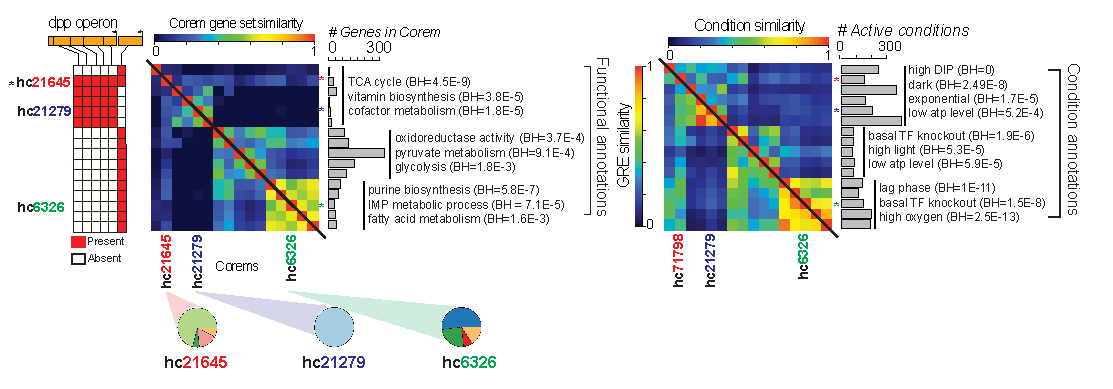
\includegraphics[width=0.95\linewidth]{figures/dpp_heatmaps.pdf}
\caption[Alternate regulatory modes for \textit{dpp} operon predicted by corems]{\textbf{\DIFaddFL{Alternate regulatory modes for }\textit{\DIFaddFL{dpp}} \DIFaddFL{operon predicted by corems.}} \DIFaddendFL Corems group together functionally related sets of genes that are co-regulated in similar environments by similar factors (Left) Presence/absence of \DIFdelbeginFL \DIFdelFL{dpp }\DIFdelendFL \DIFaddbeginFL \textit{\DIFaddFL{dpp}} \DIFaddendFL operon genes in corems. Three classes of corems exist for the dpp operon: (1) the entire operon (\eg hc21645), (2) the leader gene \DIFdelbeginFL \DIFdelFL{dppA
  }\DIFdelendFL \DIFaddbeginFL \textit{\DIFaddFL{dppA}} \DIFaddendFL (\eg hc6326), and (3) five ``tail'' genes excluding \DIFdelbeginFL \DIFdelFL{dppA
  }\DIFdelendFL \DIFaddbeginFL \textit{\DIFaddFL{dppA}} \DIFaddendFL (hc21279). (Middle) Gene similarity between corems (heatmap, Jaccard index). Functional annotations of genes in three highly similar clusters of corems to right. GRE composition for three corems shown below (pie chart, see Figure \DIFdelbeginFL \DIFdelFL{E3B}\DIFdelendFL \DIFaddbeginFL \DIFaddFL{\ref{fig:corem_gres}}\DIFaddendFL ). (Right) Similarity of conditions regulated (heatmap, upper triangle, Jaccard index) and GREs (heatmap, lower triangle, Jaccard index) among corems. Ordering is identical to (Middle). Environmental Ontology term enrichment (see \DIFdelbeginFL \DIFdelFL{Supplemental Methods}\DIFdelendFL \DIFaddbeginFL \DIFaddFL{ref}{}\DIFaddendFL ) for three clusters depicted to right.\DIFdelbeginFL %DIFDELCMD < {\bf %%%
\DIFdelFL{(C) GRE
  compositions coincide with corem membership.}%DIFDELCMD < } %%%
\DIFdelendFL \DIFaddbeginFL }
\label{fig:dpp_heatmaps}
\end{figure}

\begin{figure}[hp]
\centering
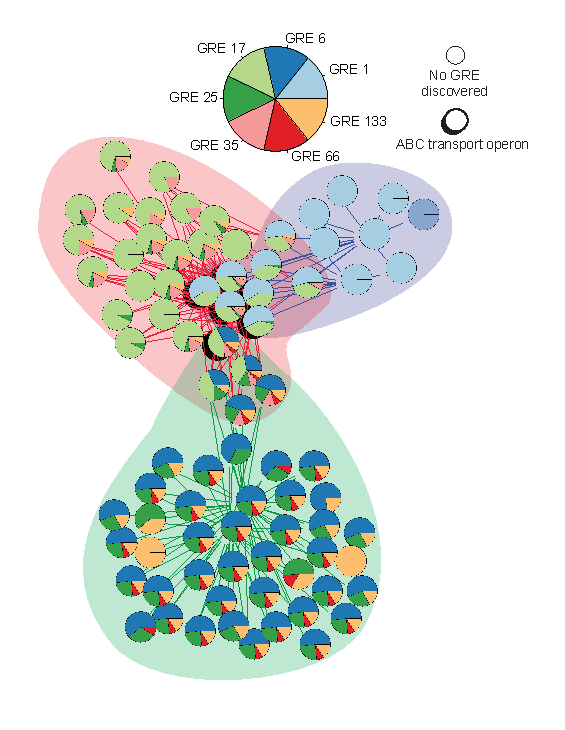
\includegraphics[width=0.95\linewidth]{figures/dpp_networks.pdf}
\caption[Network representation of transcriptional isoforms for the \textit{dpp} operon predicted by corems]{\textbf{\DIFaddFL{Network representation of transcriptional isoforms for the }\textit{\DIFaddFL{dpp}} \DIFaddFL{operon predicted by corems.}} \DIFaddendFL Network representation for three corems described \DIFdelbeginFL \DIFdelFL{above}\DIFdelendFL \DIFaddbeginFL \DIFaddFL{in \ref{fig:dpp_heatmaps}}\DIFaddendFL . Genes represented by circles. Edge colors and colored region behind the network indicate corem membership. Pie charts reflect GRE composition of each gene (see Figure \DIFdelbeginFL \DIFdelFL{E3B}\DIFdelendFL \DIFaddbeginFL \DIFaddFL{\ref{fig:corem_gres}}\DIFaddendFL ). Key for pie charts at top. Shading behind nodes (center of network) indicates \DIFdelbeginFL \DIFdelFL{dpp }\DIFdelendFL \DIFaddbeginFL \textit{\DIFaddFL{dpp}} \DIFaddendFL operon genes.\DIFdelbeginFL %DIFDELCMD < {\bf %%%
\DIFdelFL{(D) dppA is more tightly
  co-expressed with genes of hc6326 in some environments than the
  other genes in the dpp operon.}%DIFDELCMD < } %%%
\DIFdelendFL \DIFaddbeginFL }
\label{fig:dpp_networks}
\end{figure}

\begin{figure}[hp]
\centering
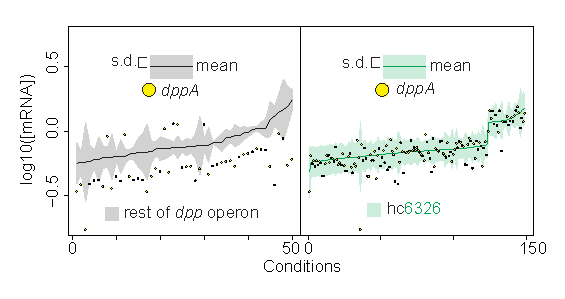
\includegraphics[width=0.95\linewidth]{figures/dpp_expression.pdf}
\caption[\textit{dppA} is more tightly co-expressed with genes of hc6326 in some environments than the other genes in the \textit{dpp} operon]{\textbf{\textit{\DIFaddFL{dppA}} \DIFaddFL{is more tightly co-expressed with genes of hc6326 in some environments than the other genes in the }\textit{\DIFaddFL{dpp}} \DIFaddFL{operon.}} \DIFaddendFL Relative expression of \DIFdelbeginFL \DIFdelFL{dppA }\DIFdelendFL \DIFaddbeginFL \textit{\DIFaddFL{dppA}} \DIFaddendFL compared to (left) other genes of \DIFdelbeginFL \DIFdelFL{dpp }\DIFdelendFL \DIFaddbeginFL \textit{\DIFaddFL{dpp}} \DIFaddendFL opeon and (right) hc6326.\DIFdelbeginFL %DIFDELCMD < {\bf %%%
\DIFdelFL{(E) EGRIN
  2.0 predicts conditional modulation of dpp operon in }%DIFDELCMD < {\it %%%
\DIFdelFL{E. coli}%DIFDELCMD < } %%%
\DIFdelFL{as
  well.}%DIFDELCMD < } %%%
\DIFdelFL{Promoter architecture within intergenic space between dppA and
  dppB suggested locations for TF binding internal to the operon (as
  in }%DIFDELCMD < {\bf %%%
\DIFdelFL{(A)}%DIFDELCMD < }%%%
\DIFdelFL{). GRE binding sites are proximal to an experimentally
  characterized IHF binding site (black horizontal bar; RegulonDB).  }\DIFdelendFL }
\DIFdelbeginFL %DIFDELCMD < \label{fig:gresVsOperons}
%DIFDELCMD < \vspace{-.1in}
%DIFDELCMD < %%%
\DIFdelendFL \DIFaddbeginFL \label{fig:dpp_expression}
\DIFaddendFL \end{figure}

\DIFdelbegin %DIFDELCMD < \begin{figure}[!b]
%DIFDELCMD < %%%
\DIFdelend \DIFaddbegin \begin{figure}[hp]
\DIFaddendFL \centering
\DIFdelbeginFL %DIFDELCMD < \epsfig{file=figures/e5.eps,width=0.95\linewidth}
%DIFDELCMD < %%%
%DIF < \\\\\vspace{.07in}\hline\\\\\vspace{.07in}
%DIFDELCMD < \caption{{\bf %%%
\DIFdelFL{4. Corems integrate and subdivide regulons and operons
    in }%DIFDELCMD < {\it %%%
\DIFdelFL{E. coli}%DIFDELCMD < } %%%
\DIFdelFL{to coordinate related biological processes.}%DIFDELCMD < }  {\bf %%%
\DIFdelFL{(A)
    Corems accurately predict conditionally modulated operons in
    }%DIFDELCMD < {\it %%%
\DIFdelFL{E. coli}%DIFDELCMD < }%%%
\DIFdelFL{.}%DIFDELCMD < } %%%
\DIFdelFL{GREs coincide with experimentally measured break
  sites. Three examples of experimentally determined transcription
  break sites (red dashed lines) in operons predicted by corems to be
  conditionally segmented. Expression levels of these regions were
  profiled across growth in rich media (heatmap). Inset contains
  region immediately surrounding a transcriptional break site,
  including counts of GREs discovered at these locations (as in Figure
  E4A). }%DIFDELCMD < {\bf %%%
\DIFdelFL{(B) Corems model the mechanistic basis for conditional
    subdivision of the PurR regulon.}%DIFDELCMD < } %%%
\DIFdelFL{(Left) Corems identify the most
  highly correlated subgroupings of genes in PurR regulon. Gene
  expression correlation across all experiments (upper triangle)
  compared to similarity of corem membership (lower-triangle, Jaccard
  index) for genes of the PurR regulon (gene identifiers expanded to
  right). (Right) Similarity of regulated conditions (upper triangle,
  Jaccard index) and GREs composition for these genes (bottom
  triangle, Jaccard index). Consistent patterns of
  conditional-activity and GRE composition in their promoter regions
  further supports subdivision of PurR genes into separate
  corems. Gene order is same as left. }%DIFDELCMD < {\bf %%%
\DIFdelFL{(C) Corems reflect
    functional integration across diverse regulatory mechanisms.}%DIFDELCMD < }
%DIFDELCMD <   %%%
\DIFdelFL{Network representation for three of the corems described above (and
  in the text). Genes are represented by circles. Edge colors and
  colored region behind the network indicate corem membership. Pie
  charts reflect GRE composition of each gene (see
  Figure~\ref{fig:fitness}B). Key for pie charts at bottom. GRE-TF
  matches are indicated. Shading behind nodes denotes PurR regulon
  genes. At least 7 different mechanisms regulate the expression of
  these genes.  }%DIFDELCMD < }
%DIFDELCMD < \label{fig:corems}
%DIFDELCMD < \vspace{-.1in}
%DIFDELCMD < %%%
\DIFdelendFL \DIFaddbeginFL 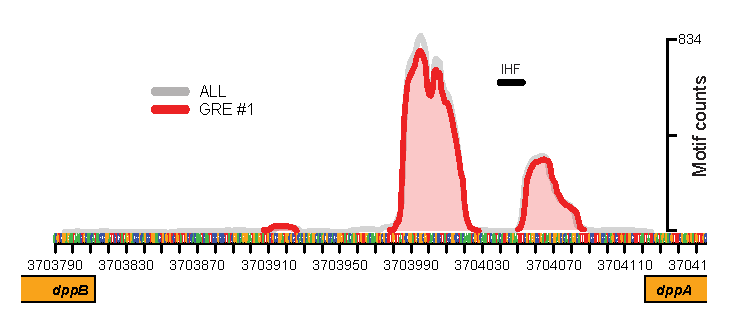
\includegraphics[width=0.95\linewidth]{figures/dpp_ecoli.pdf}
\caption[Evidence for condition-specific transcript isoforms of the \textit{dpp} operon in \textit{E. coli}]{\textbf{\DIFaddFL{Evidence for condition-specific transcript isoforms of the }\textit{\DIFaddFL{dpp}} \DIFaddFL{operon in }\textit{\DIFaddFL{E. coli}}\DIFaddFL{.}} \egrine\DIFaddFL{~predicts conditional modulation of }\textit{\DIFaddFL{dpp}} \DIFaddFL{operon in }{\it \DIFaddFL{E. coli}} \DIFaddFL{as well. Promoter architecture within intergenic space between }\textit{\DIFaddFL{dppA}} \DIFaddFL{and }\textit{\DIFaddFL{dppB}} \DIFaddFL{suggested locations for TF binding internal to the operon (as in Figure 3A). GRE binding sites are proximal to an experimentally characterized IHF binding site (black horizontal bar; RegulonDB).}}
\label{fig:dpp_ecoli}
\DIFaddendFL \end{figure}

\DIFdelbegin %DIFDELCMD < \begin{figure}[!b]
%DIFDELCMD < %%%
\DIFdelend \DIFaddbegin \begin{figure}[hp]
\DIFaddendFL \centering
\DIFdelbeginFL %DIFDELCMD < \epsfig{file=figures/e6.eps,width=0.95\linewidth}
%DIFDELCMD < %%%
%DIF < \\\\\vspace{.07in}\hline\\\\\vspace{.07in}
%DIFDELCMD < \caption{{\bf %%%
\DIFdelFL{Organization of genes in corems provides meaningful link between transcriptional regulation, metabolic dynamics and fitness.}%DIFDELCMD < } 
%DIFDELCMD < {\bf %%%
\DIFdelFL{(A) Genes from corems related to nucleotide biosynthesis have highly
  similar fitness effects when they are deleted.}%DIFDELCMD < } %%%
\DIFdelFL{(Left) Violin plot
  shows distribution of all fitness correlations for genes in three
  nucleotide biosynthesis-associated corems compared to all genes in
  the data set. (Right) KS $D$-Statistic relates to enrichment for
  highly correlated gene-gene fitness associations in the corems. All
  three corems enrich for similar fitness effects (KS FDR $< 5\times 10^{-9}$).
  }%DIFDELCMD < {\bf %%%
\DIFdelFL{(B) Corems model fitness effects that occur in specific
  environments.}%DIFDELCMD < } %%%
\DIFdelFL{Violin plots show distribution of relative fitness
  among corems across conditions (negative values indicate lower
  fitness relative to WT). Brief condition descriptions are displayed
  below. Shading within the violin plot indicates that the
  distribution of fitness values is significantly in that condition
  (KS-test FDR $\leq 0.05$). Fitness values for the subset of genes from
  the PurR regulon that do not occur in ec516031 are displayed to the
  left. These genes do not have significant fitness effects in any of
  the environments tested. Data from (Nichols et al., 2011). }%DIFDELCMD < {\bf %%%
\DIFdelFL{(C)
  Metabolite correlation explains co-regulation within
  metabolically-linked corems.}%DIFDELCMD < } %%%
\DIFdelFL{(Left) Expression correlation for TFs
  associated with three corems described in the text
  (ec516031,ec512157,ec516034). (Right) Correlation allosteric
  regulators for these TFs. TF regulated by each biomolecule listed in
  parentheses (Novichkov et al., 2010). Red boxes indicate PurR-ArgR
  and their corresponding effector molecules. Data from (Ishii et al.,
  2007).
}%DIFDELCMD < }
%DIFDELCMD < \label{fig:suppfig6}
%DIFDELCMD < \vspace{-.1in}
%DIFDELCMD < %%%
\DIFdelendFL \DIFaddbeginFL 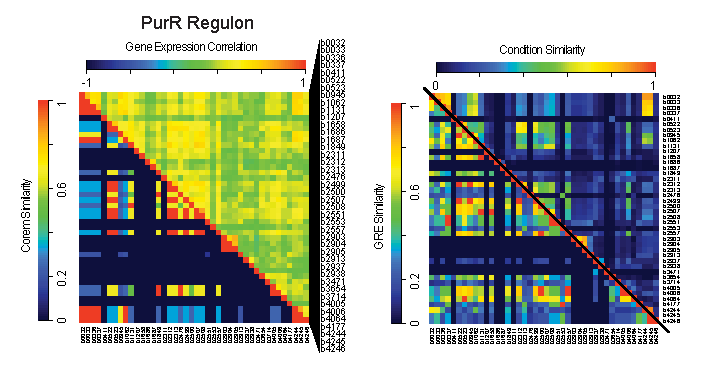
\includegraphics[width=0.95\linewidth]{figures/purR_heatmap.pdf}
\caption[Corems model the mechanistic basis for conditional subdivision of the PurR regulon, \textit{E. coli}]{\textbf{\DIFaddFL{Corems model the mechanistic basis for conditional subdivision of the PurR regulon, }\textit{\DIFaddFL{E. coli}}\DIFaddFL{.}} \DIFaddFL{(Left) Corems identify the most highly correlated subgroupings of genes in PurR regulon. Gene expression correlation across all experiments (upper triangle) compared to similarity of corem membership (lower-triangle, Jaccard index) for genes of the PurR regulon (gene identifiers expanded to right). (Right) Similarity of regulated conditions (upper triangle, Jaccard index) and GREs composition for these genes (bottom triangle, Jaccard index). Consistent patterns of conditional-activity and GRE composition in their promoter regions further supports subdivision of PurR genes into separate corems. Gene order is same as left.}}
\label{fig:purR_heatmap}
\DIFaddendFL \end{figure}
\DIFaddbegin 

\begin{figure}[hp]
\centering
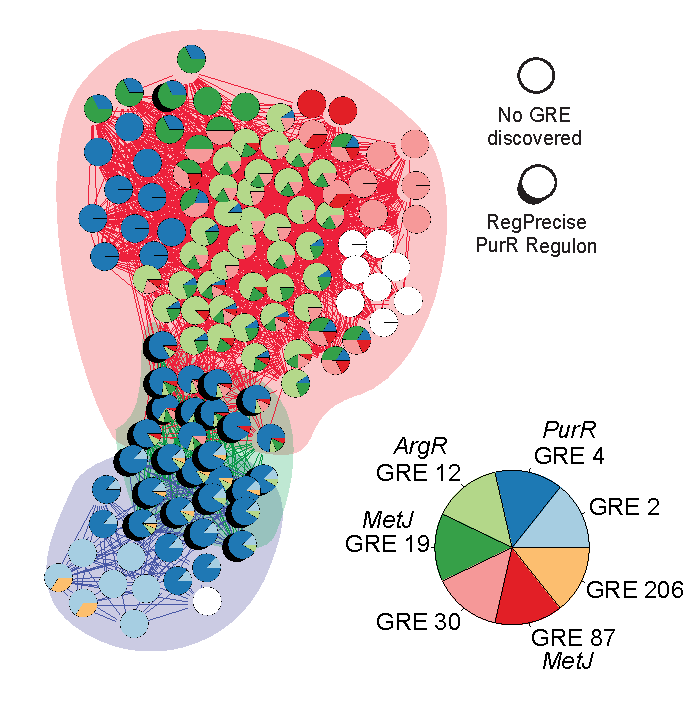
\includegraphics[width=0.95\linewidth]{figures/purR_network.pdf}
\caption[Corems integrate diverse regulatory mechanisms, \textit{E. coli}]{\textbf{\DIFaddFL{Corems integrate diverse regulatory mechanisms, }\textit{\DIFaddFL{E. coli}}\DIFaddFL{.}} \DIFaddFL{Network representation for three corems described in Figure \ref{fig:purR_heatmap}. Genes are represented by circles. Edge colors and colored region behind the network indicate corem membership. Pie charts reflect GRE composition of each gene (see Figure~\ref{fig:corem_gres}). Key for pie charts at bottom. GRE-TF matches are indicated. Shading behind nodes denotes PurR regulon genes. At least 7 different mechanisms regulate the expression of these genes.}}
\label{fig:purR_network}
\end{figure}


\begin{figure}[hp]
\centering
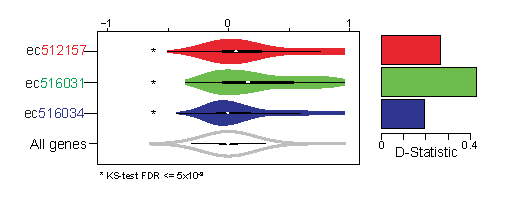
\includegraphics[width=0.95\linewidth]{figures/purR_corem_fitness.pdf}
\caption[Genes from corems related to nucleotide biosynthesis have highly similar fitness effects when they are deleted]{\textbf{\DIFaddFL{Genes from corems related to nucleotide biosynthesis have highly similar fitness effects when they are deleted.}} \DIFaddFL{(Left) Violin plot shows distribution of all fitness correlations for genes in three nucleotide biosynthesis-associated corems compared to all genes in the data set. (Right) KS $D$-Statistic relates to enrichment for highly correlated gene-gene fitness associations in the corems. All three corems enrich for similar fitness effects (KS FDR $< 5\times 10^{-9}$)}}
\label{fig:purR_corem_fitness}
\end{figure}

\begin{figure}[hp]
\centering
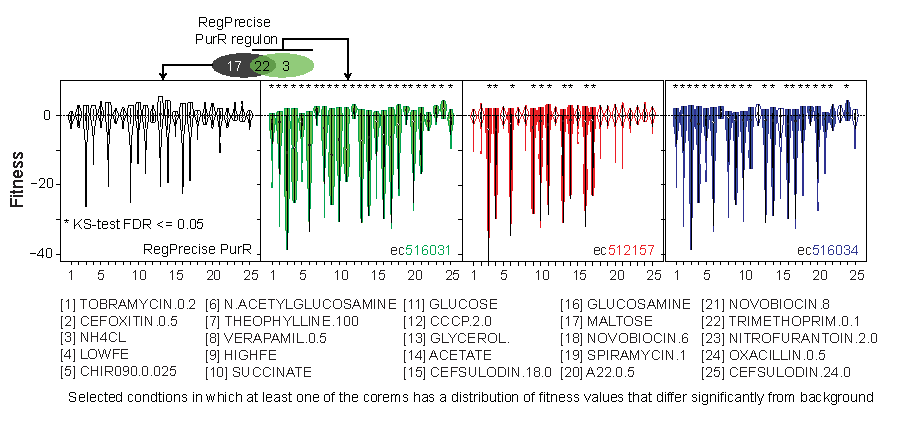
\includegraphics[width=0.95\linewidth]{figures/purR_corem_fitness_specific.pdf}
\caption[Corems model fitness effects that occur in specific environments]{\textbf{\DIFaddFL{Corems model fitness effects that occur in specific environments.}} \DIFaddFL{Violin plots show distribution of relative fitness among corems across conditions (negative values indicate lower fitness relative to WT). Brief condition descriptions are displayed below. Shading within the violin plot indicates that the distribution of fitness values is significantly in that condition (KS-test FDR $\leq 0.05$). Fitness values for the subset of genes from the PurR regulon that do not occur in ec516031 are displayed to the left. These genes do not have significant fitness effects in any of the environments tested. Data from \mbox{%DIFAUXCMD
\cite{Nichols2011}
}%DIFAUXCMD
.}}
\label{fig:purR_corem_fitness_specific}
\end{figure}

\begin{figure}[hp]
\centering
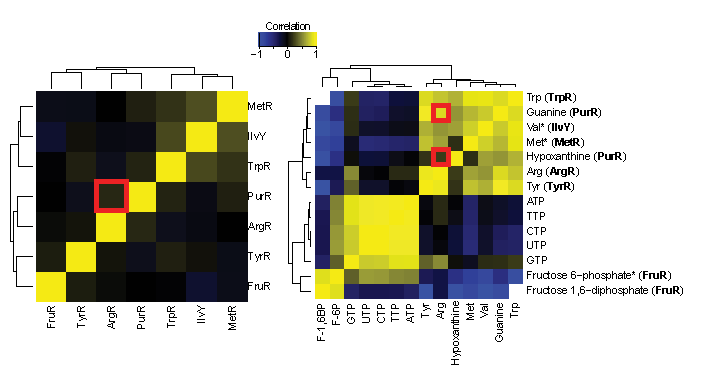
\includegraphics[width=0.95\linewidth]{figures/purR_effector.pdf}
\caption[Metabolite correlations may explain co-regulation within metabolically-linked corems]{\textbf{\DIFaddFL{Metabolite correlations may explain co-regulation within metabolically-linked corems.}} \DIFaddFL{(Left) Expression correlation for TFs associated with three corems described in the text (ec516031,ec512157,ec516034). (Right) Correlation allosteric regulators for these TFs. TF regulated by each biomolecule listed in parentheses \mbox{%DIFAUXCMD
\cite{Novichkov2010}
}%DIFAUXCMD
. Red boxes indicate PurR-ArgR and their corresponding effector molecules. Data from \mbox{%DIFAUXCMD
\cite{Ishii2007}
}%DIFAUXCMD
.}}
\label{fig:purR_effector}
\end{figure}

 \DIFaddend  %% slows it down and makes it big! Let's include it later.

\clearpage % force figures before bibliography
\bibliographystyle{abbrv}
\bibliography{egrin2_paper}{}

\end{document}
This is never printed
